% TO DO
% - Update Nominata
% - Acknowledgments
% - Improve introduction
% - Review abstract (both languages)


% 
% exemplo genérico de uso da classe iiufrgs.cls
% $Id: iiufrgs.tex,v 1.1.1.1 2005/01/18 23:54:42 avila Exp $
% 
% This is an example file and is hereby explicitly put in the
% public domain.
% 
\documentclass[cic,tc,english]{iiufrgs}

% Para usar o modelo, deve-se informar o programa e o tipo de documento.
% Programas :
% * cic       -- Graduação em Ciência da Computação
% * ecp       -- Graduação em Ciência da Computação
% * ppgc      -- Programa de Pós Graduação em Computação
% * pgmigro   -- Programa de Pós Graduação em Microeletrônica
% 
% Tipos de Documento:
% * tc                -- Trabalhos de Conclusão (apenas cic e ecp)
% * diss ou mestrado  -- Dissertações de Mestrado (ppgc e pgmicro)
% * tese ou doutorado -- Teses de Doutorado (ppgc e pgmicro)
% * ti                -- Trabalho Individual (ppgc e pgmicro)
% 
% Outras Opções:
% * english    -- para textos em inglês
% * openright  -- Força início de capítulos em páginas ímpares (padrão da
% biblioteca)
% * oneside    -- Desliga frente-e-verso
% * nominatalocal -- Lê os dados da nominata do arquivo nominatalocal.def


% Use unicode
\usepackage[utf8]{inputenc}   % pacote para acentuação

% Necessário para incluir figuras
\usepackage{graphicx}         % pacote para importar figuras

\usepackage{times}            % pacote para usar fonte Adobe Times
% \usepackage{palatino}
% \usepackage{mathptmx}       % p/ usar fonte Adobe Times nas fórmulas

\usepackage[alf,abnt-emphasize=bf]{abntex2cite}	% pacote para usar citações abnt

\usepackage{listings}

\usepackage{mathtools}

\usepackage{sepfootnotes}

\lstdefinestyle{mystyle}{frame=tb,
  language=C++,
  aboveskip=3em,
  belowskip=3em,
  xleftmargin=30pt,
  xrightmargin=25pt,
  captionpos=b,
  showstringspaces=false,
  columns=fullflexible,
  basicstyle={\small\ttfamily},
  numbers=left,
  numbersep=8pt,
  numberstyle=\tiny\color{gray},
  keywordstyle=\color{blue},
  commentstyle=\color{dkgreen},
  stringstyle=\color{mauve},
  breaklines=true,
  breakatwhitespace=true,
  tabsize=2,
  frame=single
}
\lstset{style=mystyle}

% 
% Informações gerais
% 
\title{An Implementation of Adaptive Difficulty Systems for Challenging Video Games}

\author{Tagliaro}{Leonardo Ramos Gonzalez}

\advisor[Prof.~Dr.]{Nedel}{Luciana}
%\coadvisor[Prof.~Dr.]{Knuth}{Donald Ervin}

% a data deve ser a da defesa; se nao especificada, são gerados
% mes e ano correntes
% \date{maio}{2021}

% o local de realização do trabalho pode ser especificado (ex. para TCs)
% com o comando \location:
% \location{Itaquaquecetuba}{SP}

% itens individuais da nominata podem ser redefinidos com os comandos
% abaixo:
% \renewcommand{\nominataReit}{Prof\textsuperscript{a}.~Wrana Maria Panizzi}
% \renewcommand{\nominataReitname}{Reitora}
% \renewcommand{\nominataPRE}{Prof.~Jos{\'e} Carlos Ferraz Hennemann}
% \renewcommand{\nominataPREname}{Pr{\'o}-Reitor de Ensino}
% \renewcommand{\nominataPRAPG}{Prof\textsuperscript{a}.~Joc{\'e}lia Grazia}
% \renewcommand{\nominataPRAPGname}{Pr{\'o}-Reitora Adjunta de P{\'o}s-Gradua{\c{c}}{\~a}o}
% \renewcommand{\nominataDir}{Prof.~Philippe Olivier Alexandre Navaux}
% \renewcommand{\nominataDirname}{Diretor do Instituto de Inform{\'a}tica}
% \renewcommand{\nominataCoord}{Prof.~Carlos Alberto Heuser}
% \renewcommand{\nominataCoordname}{Coordenador do PPGC}
% \renewcommand{\nominataBibchefe}{Beatriz Regina Bastos Haro}
% \renewcommand{\nominataBibchefename}{Bibliotec{\'a}ria-chefe do Instituto de Inform{\'a}tica}
% \renewcommand{\nominataChefeINA}{Prof.~Jos{\'e} Valdeni de Lima}
% \renewcommand{\nominataChefeINAname}{Chefe do \deptINA}
% \renewcommand{\nominataChefeINT}{Prof.~Leila Ribeiro}
% \renewcommand{\nominataChefeINTname}{Chefe do \deptINT}

% A seguir são apresentados comandos específicos para alguns
% tipos de documentos.

% Relatório de Pesquisa [rp]:
% \rp{123}             % numero do rp
% \financ{CNPq, CAPES} % orgaos financiadores

% Trabalho Individual [ti]:
% \ti{123}     % numero do TI
% \ti[II]{456} % no caso de ser o segundo TI

% Monografias de Especialização [espec]:
% \espec{Redes e Sistemas Distribuídos}      % nome do curso
% \coord[Profa.~Dra.]{Weber}{Taisy da Silva} % coordenador do curso
% \dept{INA}                                 % departamento relacionado

% 
% keywords
% start all keywords with lowercase letters, except in the case of acronyms
% 
\keyword{adaptive difficulty}
\keyword{dynamic content adaptation}
\keyword{player modeling}
\keyword{human-computer interaction}
\keyword{game design}

%\settowidth{\seclen}{1.10~}

% 
% Document beginning
% 
\begin{document}

% Title page
% \renewcommand{\coordname}{Course Coordinator}
\maketitle

% Abstract in the same language as the rest of the document
\begin{abstract}
    The Video Games Industry has learned through trial and error how to make digital games appeal to broad audiences. Qualities such as pleasing aesthetics, appealing story and concise playability are requirements for player engagement. However, there is a tendency for making games easier to support entry-level players. While this is a respectful approach to embrace casual players, it might bore skillful players which dedicate more time to gaming. One interesting solution to this problem is the concept of "adaptive difficulty". Instead of reducing difficulty curves to finite menu options such as "Easy" and "Hard", difficulty is treated as a set of in-game continuous variables in multiple layers, each pertaining to a specific set of the game's rules. The game monitors player actions and their results to dynamically adjust in-game parameters and tailor the difficulty of game systems to the specific needs of a player. Therefore, the player does not have to manually input their desired difficulty level, and the game smoothly adapts to the player's profile. We review multiple dynamic difficulty methods proposed in commercial games and in prior academic work, and present an implementation of player-centric adaptive technology in games. We evaluate the benefits of personalizing the game based on user preferences and performance, using the \emph{Dark Souls} game series as an object of study. We implement a subset of the \emph{Dark Souls} game mechanics with a simplified version the features presented in the original game. The customization methods include dynamic and subtle gameplay changes, a Dynamic Difficulty Adjustment system and a player model based approach for performance tracking.
\end{abstract}

% Second language abstract
% Parameters must include the title and keywords
% in the other language, separated by commas
\begin{englishabstract}{}{Dificuldade adaptativa. adaptação dinâmica de conteúdo. criação de modelo de jogador. interação humano-computador.}
    A indústria de video games aprendeu, por tentativa e erro, como fazer jogos serem atraentes para um público grande. Estética agradável, uma história envolvente e jogabilidade concisa são características necessárias para engajar o jogador. No entanto, existe uma tendência em fazer com que jogos não sejam desafiantes para que sejam acessíveis a jogadores novatos. Enquanto que esta solução respeita a as necessidades de jogadores casuais, jogadores mais habilidosos que dedicam mais tempo a jogos podem se sentir entediados e desmotivados a jogar. Uma solução para este problema é o conceito de "dificuldade adaptativa". Ao invés de tratar dificuldade como um número finito de opções de menu nomeadas "Fácil" e "Difícil", a dificuldade é tratada como um conjunto de variáveis contínuas em múltiplas camadas, cada uma representando um conjunto de regras do jogo. O jogo monitora as ações do jogador e seus resultados, de forma a ajustar os parâmetros do jogo para se ajustar ao perfil de dificuldade do jogador. Portanto, neste trabalho apresentamos uma implementação para adaptação dinâmica de conteúdo em jogos centrada no jogador, e avaliamos os benefícios causados pela adaptatividade baseada em preferências e performance do usuário. O objeto de estudo é uma implementação de jogo inspirada no título \emph{Dark Souls}, com um conjunto reduzido e simplificado de mecânicas do jogo original. Os métodos de personalização incluem mudanças sutis na jogabilidade baseadas em preferência, um sistema de Ajuste de Dificuldade Dinâmico e mudanças no ambiente baseadas em estado de jogo.
\end{englishabstract}

%\renewcommand{\abstractname}{Acknowledgments}
\chapter*{Acknowledgments}

%\begin{flushright}
%     \mbox{}\vfill
%     {\sffamily\itshape
%       ``This is a quote,\\
%       said by an important author.''\\}
%     --- \textsc{Important Author}
% \end{flushright}

% List of Figures
\listoffigures

% List of tables
\listoftables

% List of listings
% \lstlistoflistings

% List of abbreviations and acronyms
\begin{listofabbrv}{SPMD}
    \item[2D] Two-dimensional
    \item[3D] Three-dimensional
    \item[ADC] Adaptive Duo-Chromosome Controller
	\item[AGT] Adaptive Game Technologies
	\item[AI] Artificial Intelligence
	\item[API] Application Programming Interface
	\item[AUC] Adaptive Uni-Chromosome Controller 
    \item[DDA] Dynamic Difficulty Adjustment
    \item[ECG] Electrocardiogram
    \item[EMG] Electromyography
    \item[HCI] Human-Computer Interaction
    \item[HMD] Head-Mounted Device
    \item[NPC] Non-Player Character
    \item[RPG] Role-Playing Game
    \item[RT] Regression Tree
    \item[UX] User Experience
    \item[VR] Virtual Reality
\end{listofabbrv}

% List of symbols
%\begin{listofsymbols}{$\alpha\beta\pi\omega$}
%    \item[$\sum{\frac{a}{b}}$] First symbol
%    \item[$\alpha\beta\pi\omega$] Another symbol
%\end{listofsymbols}

% Contents
\tableofcontents

%============================================================
%============================================================
%============================================================
%============================================================
%============================================================
%============================================================

\chapter{Introduction}

Game Designers are often riddled by the trade off of either appealing to the largest audience possible or entertaining the preferences of a niche. When creating games for a broad audience, game designers lean towards the preferences of casual players, using predefined and well-known features to take advantage of popular features that trend in a game genre. When creating niche games, designers often express more freedom, exploring new features, mixing older ones and creating complex systems that are well received by the target audience. This can be seen in complex Role-Playing games such as \emph{Path of Exile} \footnote{Path of Exile (Grinding Gear Games, 2013). Computer Game. Microsoft Windows.} or \emph{Diablo} \footnote{Diablo (Blizzard Entertainment, 1996). Computer Game. Microsoft Windows.}.

Tailoring a game to a specific niche during the conceptual phase of development is a valid approach to solidifying its core characteristics. However, in the last decades there has been an increasing interest in making games versatile to multiple audiences, creating flexible layers of content and adapting to different types of players during the act of play. Different types of players have specific needs, and will find enjoyment in specific characteristics of a game such as aesthetic preferences, narrative types and challenges.

In a general sense, for a game to successfully bring enjoyment the player has to be involved and focused while playing. Therefore, one of the critical factors of a game's success is its ability to make the players immersed in its experience, which might occur in a way that is a deviation of a game designer's intention. The most established concept in academic literature pertaining player immersion and focus is the theory of Flow \cite{BOOK_Flow}. 

Flow is the state in which a player is completely immersed within the experience of a game. The ease to reach the state of Flow is determined by, among other properties, the challenge of a game in contrast to the skill of its player. According to the Theory of Flow, for a player to become completely immersed the difficulty of the game should match their skill \cite{ARTICLE_FlowInGames}. A game that is not challenging at all will bore the player. A game that is too challenging might cause anxiety and result in the player giving up. 

A game with balanced challenge for all players would ideally be the best solution. In practice it is difficult to accomplish, risking an unsatisfactory result for each type of audience. However, as seen in \cite{ARTICLE_PlayerCentredGameDesign}, it is possible to adapt a game in real time to satisfy the needs specific to the preferences of a player. Such a model can be achieved through AGT (Adaptive Game Technologies), where the game application learns the user profile and adapts its content to provide a dynamically customized experience.

The customized experience might be represented by content tailored to the preferences of a player, such as a specific type of mission that is assigned to the player. An example would be a stealth mission to a more strategic player, requiring the player to traverse the environment carefully. In contrast, for a player that enjoys action, a mission involving chaotic gunfire and explosions might be more aligned with their needs.

This work is an implementation and analysis of a simplified replica of a successful hardcore niche game, \emph{Dark Souls}, using AGT to appeal to a broader audience. The application creates a Player Model based on user-provided information, adapts its content through statistical gameplay data obtained by telemetry and allows the user to experience the game with an appropriate difficulty curve by dynamically adapting the challenges presented on each level.

\begin{figure}[!h]
    \caption{A screen capture of our implementation of a \emph{Dark Souls}-based game with a subset of the features present in the original game.}
    \begin{center}
        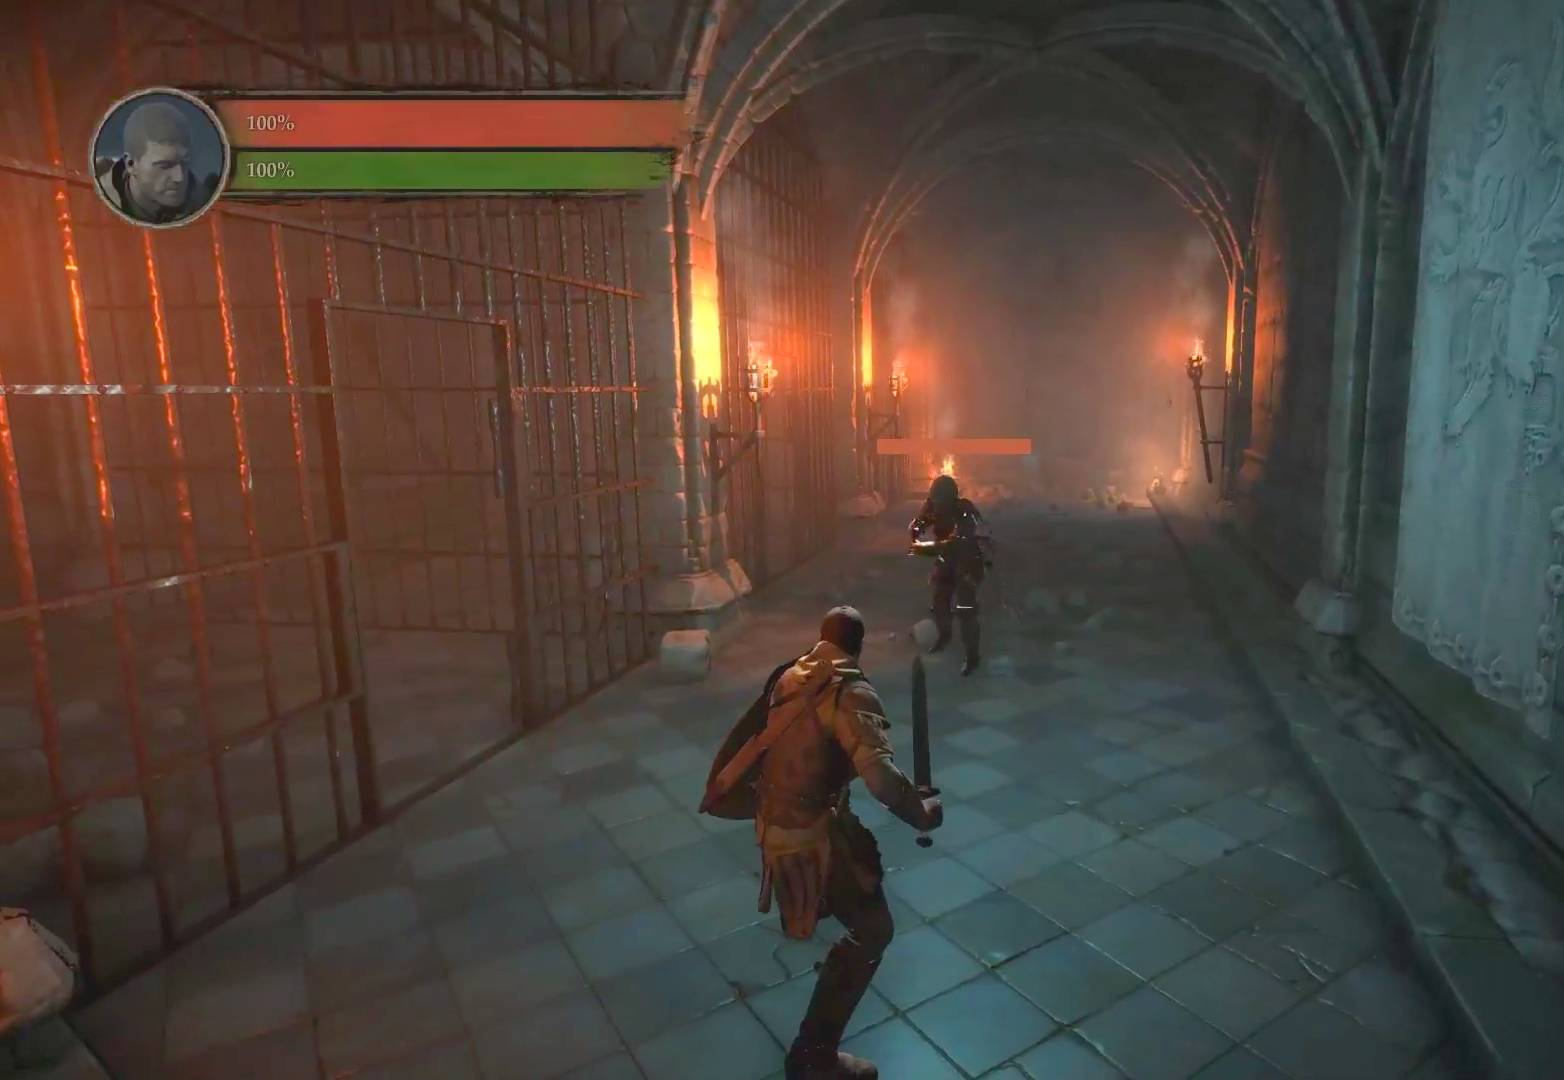
\includegraphics[width=26em]{figures/fig-bright-souls.jpg}
    \end{center}
    \legend{Source: Screen capture performed by the authors on a Microsoft Windows system.}
    \label{fig:ex1}
\end{figure}

To replicate the scenario of a successful commercial game, we look at how the problem of adaptive difficulty  is handled in multiple commercial games. Then, we analyze in depth the aspects that contribute to the difficulty of \emph{Dark Souls}, and attempt to replicate them in a simplified implementation. We compare the implementation of our solution to the original game, and outline the gameplay features that constitute the \emph{Souls}-like experience.

We propose a possible method for the design, implementation and usage of AGT as means of enhancing player experience. We compare the results in presence and absence of AGT, using as parameter a user evaluation on their perceived experience for each scenario and performance analysis based on gameplay data.

%============================================================
%============================================================
%============================================================
%============================================================
%============================================================
%============================================================

\chapter{Related Work}

In this chapter, we evaluate the early solutions to adaptivity in commercial games, analyzing their positive and negative aspects. We explore the concept of Player Modeling, an attempt at defining player profile and preferences as functional data that can be used by game applications as input for multiple systems. We relate the concept of player models to the ever increasing research in game analytics, where player behavior is monitored and used as a tool to identify game design issues and improvements that directly affect player engagement.

In conclusion, we review previous research on AGT \cite{ARTICLE_PlayerCentredGameDesign}, the solution that proposes to enhance user experience based on player profile and preferences. We argue that AGT can be used to alleviate the steep learning curve of highly challenging games, accommodating the skill level beginner players to the challenge designed by game developers.

\section{Overview}

\subsection{A Timeline of Adaptive Game Systems}

\subsection{A Comparative Table of Research in Adaptive Game Systems}

\section{Adaptive Systems in Commercial Games}

Several commercial games have attempted to create Dynamic Difficulty systems which embrace varying degrees of player skill, such as \emph{Mario Kart} \footnote{Super Mario Kart 8 Deluxe (Nintendo, 2017). Video Game. Nintendo Switch.}, \emph{Half-Life 2} \footnote{Half-Life 2 (Valve Software, 2004). Computer Game. Microsoft Windows.}, \emph{Resident Evil 4} \footnote{Resident Evil 4 (Capcom, 2004). Video Game. PlayStation 2.} and \emph{God Hand} \footnote{God Hand (Capcom, 2006). Video Game. PlayStation 2.}. In this section, we look at examples of Adaptive Systems in some of the most popular games developed by the video game industry in the last decades. We categorize the solutions based on which game systems they affect, and discuss some of the caveats of each system.

\subsection{Rubber-banding in Mario Kart}

Perhaps the most popular approach to Adaptive Difficulty is found in games which present \emph{rubber banding}. This technique is most commonly seen in racing games that have artificial intelligence agents as opponents to the player. If the player performs exceptionally well in a race and is far ahead of every AI opponent, the opponents will receive a significant speed boost that often surpasses the standard speed limits of the game. In case the player performs poorly, the AI is slowed down below their base speed so that the player is able to catch up. The term \emph{rubber banding} derives from the analogy that the players and their opponents are held together by a rubber band, so that they are never too far apart from their opponents.

Rubber banding is employed to cause the impression that the outcome of the race is never clearly defined, enabling the perception that mistakes by the competitor that is ahead can greatly affect their chances of winning. The existence of the rubber banding system, along with the perception caused by it, results in the increase of tension and focus by the player. Rubber banding is not limited to the Racing games genre, and it does necessarily happen only between players and AI. However, it does imply that the game has some sort of competition system, even if the game is a single-player \footnote{A single player game is a video game where the input processed by the game is received from only one human user (player) during the course of a game session. All entities the player interacts within the game world are non-player entities.} or cooperative \footnote{Cooperative games are games in which the input is received from multiple human users (players), with each player controlling a different in-game entity. The players share a common objective, and must cooperate by combining their available commands and actions to achieve the winning condition.} experience.

Mario Kart applies rubber banding through two different methods, affecting both players and computer-controlled opponents \cite{website_rubberbandingmariokart}. The first type of rubber banding compares the performance of players to AI opponents: if a player is too far behind the computer-controlled opponents, the AI slows down by lowering their maximum speed. If a player is too far ahead, the AI receives a significant speed boost to their base speed. While being a simplistic solution common to many games in the racing genre, it attenuates the skill discrepancy between players and AI. 

The second solution in Mario Kart is presented through the power-up system, and targets the issue of skill discrepancy between players. Throughout the race, players are provided with multiple randomly-generated power-ups, which can be used to speed-up, attack or defend against opponents. Speed-up pickups are favored to players who are far behind others, whereas attack and defense power-ups are favored to players who are closer to attaining the first position. Players in the first position are generally provided the worse pickups. This provides better opportunities for players who are lower-skilled, as the access to speed power-ups is limited to the competitors who are far behind, and effectively serves as a catching-up mechanic.

While this solution is an interesting and creative effort that makes matches between players of varying skill levels more competitive, players that become aware of this system might avoid the first position to retain the best power-ups until the last moments of a race. This situation elicits the problem of meta-gaming in adaptive systems: when the adaptive systems are well-known by the users, exploits become a part of player strategy.

\subsection{Dynamic Enemy Behavior and Encounters in Resident Evil 4}

Another interesting approach to adaptivity is seen in Resident Evil 4, where level design, AI behavior and item distribution systems are affected by player performance. Resident Evil 4 presents three layers of gameplay adjustments controlled by a DDA system: Dynamic Enemy Behaviors, Dynamic Encounters and Dynamic Item Distribution. Each layer attempts to satisfy player needs according to a set of conditions related to gameplay context.

One example of such conditions is the player having a low amount of health points and no health sustain resources in their inventory, where the Dynamic Item Distribution layer will affect health resource distribution by modifying the chances of containers or defeated enemies containing health recovery items upon interaction.

Therefore, the Dynamic Item Distribution layer interferes with the random generation of items. If the player is not in a risk situation or has a lot of ammunition, the game will often prioritize gold coins, which can be used to purchase powerful weapons and weapon upgrades.  Veteran players that are aware of this system attempt to maintain their resources at a controlled level, so that the most important resources are distributed at critical points in the game campaign, such as before an encounter with a large group of enemies.

The Enemy Behavior layer affects the behavioral aspect of AI-controlled entities in relation to player skill. If a player is able to defeat enemies easily by shooting their heads or without spending significant resources such as ammunition and health recovery items, enemies will start to perform new actions such as attempting to dodge or even using their hands to block bullets. Therefore, enemy behavior changes according to player precision and effectiveness.

Although the new actions can prove to be an obstacle for player effectiveness, they are not overwhelmingly difficult to handle. An experienced player can still be effective and shoot enemy heads with precision if they are able to predict enemy movement or quickly react to the new character animations. Therefore, the game increases its skill ceiling[Footnote: What is skill ceiling] and enables interesting situations in enemy encounters even for experienced and highly skilled players. 

Resident Evil 4 uses a skill rating system called \emph{Game Rank}, which is increased or decreased according to aim precision and level completion time [Reference: JP RE4 Strategy Guide Pages 23-26]. Veteran players and \emph{speedrunners}\footnote{Speedrunners are players which attempt to complete games in the least amount of time possible, and often compete in online leaderboards for ranking themselves among the fastest completion times. There are many online speedrunning communities which enforce a set of rules to ensure the validity of a run, including video proof and the absence of cheats.} are able to exploit this rating value by missing shots on purpose, artificially lowering their precision value and Game Rank. This causes the game to constrain enemy behavior to predictable movement patterns, where shooting enemy heads is easier than in a standard play through. This is another example of meta-game strategies in adaptive solutions, where players that are knowledgeable of the adaptive systems attempt to explore it to constrain the behavioral patterns of AI agents.

The Dynamic Encounters layer tackles the placement of enemies in levels, affecting the difficulty of specific encounters. If the player repeatedly dies in some sections of the game, certain enemies spawns are disabled, making the encounter much less frustrating. In general, long range enemies such as crossbow wielders which are hard to reach or take a longer amount of time and resources to eliminate are the first to be disabled since there is no direct or easy method for the player to avoid them. Also, since the game was originally planned for exclusive console release, it is only natural that long-range enemies require more input precision to be dealt with, due to the nature of Joystick controllers[Footnote: What are joystick controllers].

Another instance of the Dynamic Encounters layer changing level layout is seen in with ambush-type enemies, which will only spawn outside of player field-of-view. Since these enemies are harder to perceive, they will often be harder to react to and force the player into quick decision-making. If the player is performing well and accumulates a significant amount of health resources, ambush-type enemy spawns are enabled to cause the perception that even though the player is skilled enough to deal with enemies in direct combat, there are still traps and surprising situations that might cause the player to be defeated.

While Resident Evil 4 received mass critical praise for its outstanding game design and successful adaptive approach, it is noteworthy that a community of dedicated \emph{speedrunners} has been able to accurately reverse engineer and exploit its DDA systems [Footnote: Speedrun.com Resident Evil 4 Guides]. It can be argued that given enough dedication, there is no DDA system which is completely unknown to players. However, since the reverse engineering process requires extensive experimentation on behalf of players, we can assume that the system will remain mostly obfuscated to novice players experiencing their first play through, which is critical to maintain immersion and player engagement.

\subsection{Explicit Adaptivity in God Hand}

In \emph{God Hand}, the developers approached the adaptivity issue explicitly by making the player constantly aware of the difficulty level \cite{article_subjectivedifficulty}. A difficulty meter is presented to the players containing 3 difficulty levels. Whenever the player hits an enemy, the meter slightly increases. When the meter is full, the difficulty level is incremented and enemies become faster, smarter and deal more damage.

When difficulty is maxed out, enemies hit faster than the player character is able to dodge. Thus, to beat the highest level of difficulty the player must devise a strategy and perfectly execute all their attacks. Whenever the player beats and enemy, they are rewarded with an amount of points and coins based on the current difficulty level. When the player takes damage, the difficulty level is decreased. This solution is especially interesting to anticipate frustration caused by players being aware of adaptivity. 

Instead of hiding the system, the developers of God Hand encouraged players to play at their highest skill level. Increasing the difficulty level also increases the amount of rewards, and creates a sense of achievement for winning at unfair odds. In this case, it can be argued that the game revolves around its Dynamic Difficulty System, in the sense of the player feeling accomplished whenever they can maintain a long streak of encounters in the highest difficulty level. 

This is a particularly interesting take on the issue of players feeling cheated or without control of their experience. In God Hand, players will push their skills to the limit to maintain the highest difficulty possible for as long as possible. Therefore, players know that if the game becomes too slow, it is a product of their own skill and decision-making.

\section{Research on Dynamic Difficulty Adjustment Systems}

Mechanisms for DDA should describe what elements of the game are going to be monitored, and what variables should be adjusted accordingly. Therefore, the functionality of a DDA system can be summarized as a relation between observation and adjustment. Since video games are so diverse in design and functionality, the mapping between observation parameters and adjustment variables has yet not been efficiently described as an universal and generic approach \cite{PHD_DynamicDifficultyAdjustment}. Rather, the game developer should decide what variables should be observed and adjusted in a per-game basis.

In contrast to the implementations of DDA portrayed in commercial games, prior academic work encompassed a multitude of probabilistic models and data-driven approaches that could prove to be interesting if applied to a commercial solution. In the scope of this work, we use the literary review in \cite{article_ddareview} as a reference to categorize a subset of DDA algorithm variants implemented in previous academic work, as well as to select and perform an analysis on a single relevant representation for each of the proposed solutions.

\subsection{Probabilistic DDA Systems}

One of the first and most relevant implementations of the probabilistic model approach for DDA systems is the Hamlet system seen in \cite{article_casefordynamicdifficulty}. Hamlet is a probability-based predictive system that is able to perform reactive and proactive adjustments to the distribution of items throughout levels of customized Half-Life \footnote{Half-Life (Valve Software, 1998). Computer Game. Microsoft Windows.} map \cite{article_casefordynamicdifficulty}. The system works by defining a finite set of possible game world states, and performing adjustments with the objective of avoiding game state "loops", where a player would perform the same set of actions repeatedly.

First, Hamlet establishes the probabilistic distribution of damage done to the player using a series of measurements taken over time. By doing this for each of the enemy classes, the probability of the player dying during an encounter can be estimated. Then, if the probability of death for an encounter is above 40\%, the system intervenes by distributing \emph{healing items}\footnote{Healing items in games are consumable resources that restore a percentage of the maximum health points of a player. An example for this are the health stations in the Half-Life franchise, where the player heals up to 80\% of their maximum health points upon interaction, but the resource is permanently depleted after use.} throughout the level before an encounter takes place. This is an example of \emph{proactive adjustment}, which occurs before an in-game event takes place. The author of the article argues that the effectiveness of proactive adjustments is harder to measure than \emph{reactive} adjustments, and thus this type of adjustment should be performed based on predefined constraints determined by the game designer.

Hamlet is also able to perform \emph{reactive} adjustments that occur during combat encounters, such as adjusting the maximum hit points for an enemy class or modifying the accuracy of enemy shots. The objective of any adjustment is to decrease the amount of player deaths for each level independently of player skill, and to achieve a mean health percentage of 60 with a standard deviation of 15 points at any given point.

Results of the experiment using the Hamlet system showed that most players were unable to recognize when the system was performing adjustments, or characteristics of the game were modified when adjustments were performed. Some players suggested that the system performed adjustments that were not there, and several players suggested that the system did not perform any adjustments based on their skill level. During the post evaluation interviews, there was a slight correlation between the adjustment policies and player enjoyment when considering players with expert skill level, although players with novice skill level did not report any perceivable change.

The study concluded that adjustment algorithms can include the performance of a player while retaining the player's sense of agency and control. When performed with accordance to the game's core design, adjustments can be nearly imperceptible, and slightly increase the sense of enjoyment of a player without diverging from the proposed experience.

Therefore, the Hamlet system proposed by \citet{article_casefordynamicdifficulty} addresses the possibility of predicting gameplay outcomes given a game world state, and performing \emph{reactive} or \emph{proactive} adjustments for a more immediate resolution when compared to other solutions. We argue that while this might be an interesting approach for a supportive or secondary DDA system, this type of solution might be hard to tailor from a game designer's perspective since it is impossible to predict results functionally.

\subsection{Affect-based DDA Systems}

Most implementations of DDA systems use as adjustment policies metrics that would represent player performance. However, the affective state experienced by players could also play a key role in the gaming experience, and thus could be a useful metric for adjustment policies in DDA systems. This is the theme of the work presented in \cite{article_affectivedda}, where physiological signals were tracked to infer the anxiety level of players, and then used as a metric to perform dynamic adjustments.

The work of \citet{article_affectivedda} cites previous research indicating that electrodermal and cardiovascular activities had a relation to anxiety levels. An increase in skin conductance may be caused by anxiety. A decrease of parasympathetic activity and increase in sympathetic activity in the heart also may suggest anxiety \cite{article_affectivedda}.

Blood pulse volume measured at fingers were also shown to be subject to stress manipulation, and presents a correlation with self-reported anxiety \cite{article_affectivedda}. Measures of EMG (Electromyography) activity of specific muscles (such as Corrugator Supercilii) were also shown to be strong indicators of anxiety.

Therefore, the work presented in \cite{article_affectivedda} used features of cardiovascular activity, such as interbeat interval, relative pulse volume, pulse transit time and heart sound; electrodermal activity (tonic and phasic response to skin conductance) and EMG activity (from Corrugator Supercilii, Zygomaticus and upper Trapezius muscles) as input measures to a Regression Tree (RT) technique which classifies the physiological signals into affective states that categorize anxiety levels.

A Pong-based game was implemented for the study, with two variations in difficulty adjustment algorithm: one where the difficulty would be adapted based on player performance (a relationship between points scored against or in favor of the player), and another where the anxiety level of the player is used as input to alter difficulty.

Three difficulty levels were implemented in total, which would be assigned depending on performance or anxiety levels: if the player's performance is classified as "Excellent", the player would progress into the next difficulty level. If the performance is classified as "Poor", the difficulty level would be decreased. The affect-based variant utilizes an analogue solution, where the difficulty is increased if the anxiety level is classified as "Low", and the difficulty is decreased if the anxiety level is classified as "High". Figure \ref{fig:affective-adaptation} displays state-flow diagrams representing the difficulty levels and their transition conditions.

\begin{figure}[!h]
    \caption{A state-flow diagram representation of the performance-based and anxiety-based adaptation variants in \cite{article_affectivedda}.}
    \begin{center}
        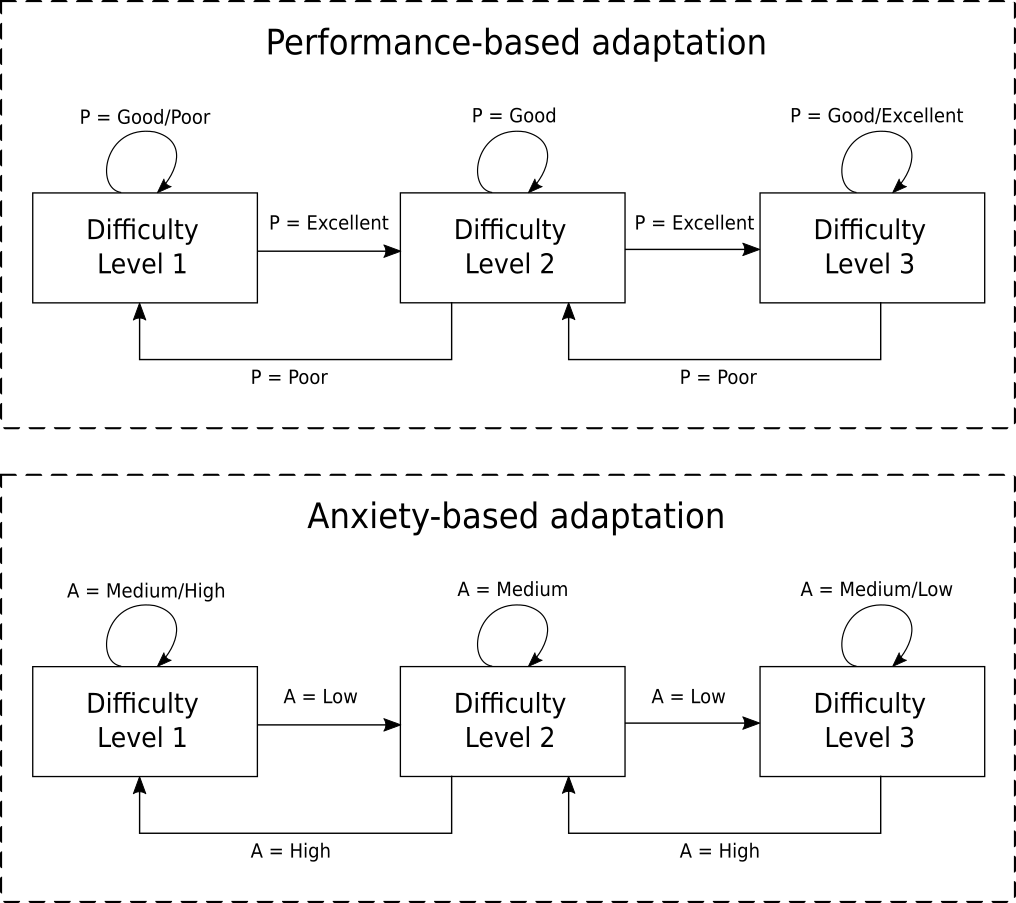
\includegraphics[width=26em]{figures/fig-affective-adaptation.png}
    \end{center}
    \legend{Source: Diagram assembled by the authors based on visual representations in \cite{article_affectivedda}.}
    \label{fig:affective-adaptation}
\end{figure}

The results of the experiment showed that the performance of most players improved during the affect-based DDA session in relation to the performance-based DDA session. Players also perceived the affect-based DDA version to be more challenging than performance-based DDA, and reported that the affective version was more satisfying.

We argue that, while the results of the experiment portrayed in \cite{article_affectivedda} showed mostly positive results in comparison to performance-tracking DDA, employing this type of solution in a commercial video game is not feasible, as current hardware is unable to track physiological signals in a significant way. 

Furthermore, the game implementation used for the experiment is a simplistic game with limited audiovisual feedback. Therefore, a similar experiment could be performed in a modern game with high audiovisual fidelity to evaluate results, as modern games are often able to evoke a multitude affective reactions by immersing the player in a \emph{cutscene}\footnote{A \emph{cutscene} is a special in-game event where the player is unable to input control into the game, and audiovisual feedback is a result of an automatic, predefined sequence of events determined by the game developers. Cutscenes can be seen as parts of a game that are similar to a movie, where the game is not interactive and instead focuses on telling a part of the story.} or a series of chaotic events.

\subsection{Reinforcement Learning in DDA Systems}

Another approach to adaptive difficulty involves the adaptation of AI (Artificial Intelligence) agent behaviors through reinforcement learning, as exemplified in \cite{article_adaptivebehaviorai}. Their implementation defines AI agents in a simple car simulation race game, where each player has the objective of passing through the maximum number of \emph{waypoints}\footnote{A \emph{waypoint} is a special position in a game world where an in-game event is toggled when the player is within interaction range. Waypoints are commonly used in games when the player has to take a specific path to a goal, with the game assigning several intermediary positions the player has to pass through to validate that the correct path was taken. In the context used for the implementation presented in \cite{article_adaptivebehaviorai}, waypoints are simply game world positions the cars must reach to score points. Each time one of these positions is occupied by a car, the waypoint is destroyed and a new random position is assigned elsewhere in the game world as the next waypoint.} in a given amount of time. Multiple waypoints are displayed on the screen at any given time, and a waypoint disappears when any of the players is within interaction range.

The AI agents implemented in \cite{article_adaptivebehaviorai} define two layers of behavioral AI components. The first layer contains components associated with driving functionality, with the objective of improving driving performance of the controller. The second layer is associated with tactical behavior components that seek to outplay the opponent in the game.

Driving behavior components ignore the existence of the opponent, leading to inferior performance in the game. Tactical behavior components help the AI controller decide which waypoint to head to, or if the controller should not head to a waypoint at all. In more general perspective, the Driving Behavior components can be seen as the mechanical input of AI agents in the game, whereas the Tactical Behavior components could be considered the high-level decision making components of the AI.

To evaluate the performance of adaptive AI agent controllers, two evolutionary computation algorithms are implemented: the adaptive uni-chromosome controller (AUC) and the adaptive duo-chromosome controller (ADC). The advantage of using such algorithms is that the training and adaptation process occurs in real time during the course of a game session.

Each chromosome in said algorithms stores seven real numbers representing the probability of activating a behavioral component whenever a waypoint is passed. Two metrics are used as an input for the adaptation algorithm: first, a minimization of the winning percentage difference (|W - L|, where W represents the wins and L represents the losses) and second, a minimization of the mean score difference (|s1-s2| where s1 and s2 represent the scores of player 1 and player 2).

To evaluate the efficiency of the proposed algorithms, the authors first compared the strongest AI agent that the adaptive system would possibly generate (defined by enabling all behavioral components simultaneously and permanently) against five static AI controllers based on various traits that would simulate various styles of play, such as heuristic controllers, reverse-enabled controllers, predictive fast controllers, and neural network controllers.

Sets of \emph{n = 5000} games were played for each opponent in each step of the experiment. Through the first step of the experiment, the authors validated that a fully-enabled adaptive AI controller (having all the behavioral components activated at all times) was a competent opponent with positive median score differences against all static AI controllers.

In the second step, the behaviors were activated randomly whenever a waypoint was crossed to demonstrate that an effective adaptation algorithm is necessary for different types of oponents. Results showed that the random behavior selection algorithm had negative median score differences against all five static controllers.

In the third step, the authors evaluate the use of the AUC algorithm. The expected behavior set encoded by a chromosome as a result of the algorithm should represent a "winning" strategy. Effects of varying \emph{Learning Rate}\footnote{Learning Rate: [FN]} and \emph{Mutation Rate}\footnote{Mutation Rate: [FN]} were documented for the experiment, showing that the general trend of increasing learning rate is a gentle increase in the mean score difference, since a large learning rate quickly saturates chromosome values to either 0 or 1. Higher mutation rates tend to produce larger differences in mean score and winning percentage by producing large fluctuations in chromosome values. In general, high mutation rates led to poorer results, and the optimal value of 0.1 was stated for the AUC algorithm variant.

In the final step of the experiment, the use of the ADC algorithm is evaluated, with the same idea of varying the Learning and Mutation Rates. For the ADC algorithm, no trends were perceived in association with varying Learning rates. This would likely have been caused by the reduction of the frequency of update opportunities for each chromosome. In the ADC algorithm, only one of two chromosomes is updated each time a waypoint is passed. This means that on average each chromosome is updated half as frequently as chromosomes in the AUC variant. As for the Mutation rate, the results of the ADC controller improved greatly as mutation was introduced, possibly because the mutation operation offered more opportunities for the chromosome values to adapt.

As a conclusion to the experiment, the authors expressed that while the AUC algorithm had lower memory footprint, the ADC algorithm was able to better minimize the number of drawn games, which would possibly reduce player frustration. It was also noted that both the AUC and ADC algorithms were able to generate specific patterns of behavioral component distribution for each of the static controller stereotypes, meaning that the Reinforcement Learning technique would be able to adapt to different styles of play. The general intent of both algorithms was not to maximize the number of wins, but to maintain a fair and close challenge to the opponent by minimizing the score difference as well as the difference between number of wins and losses.

The work presented in \cite{article_adaptivebehaviorai} introduces the novelty approach of online learning without predefined data sets to the scenario of DDA solutions. It could be argued that the adjustment policies are also part of the reinforcement learning approach, since the decision of a behavioral component being activated or not relies on the algorithm being applied. This is an especially interesting solution since it lessens the responsibility of a game designer tailoring the boundaries of the adjustment system in advance of play. However, we argue that this experiment has yet to be applied in the context of real players using an implementation that would better replicate a commercial video game product.

\section{Player Modeling and Profiling}

The concept of adaptivity in games relates to how a game is able to adapt its content based on the \emph{profile}\footnote{Player profile: [FN]} and \emph{preferences}\footnote{Player preferences: [FN]} of a player, which constitute \emph{player models} obtained from a multitude of \emph{Player Modeling} techniques.

Player Modeling allows creation, collection and processing of \emph{player models}, real-time collected data sets that can be classified into reality-based player types \cite{ARTICLE_DynamicPlayerModelling}. Knowledge about player types allows dynamic adjustment in the sense of content customization, where a game designer might dynamically assign what should be presented to each type of player.

In a DDA system, \emph{Player Models} refer to collections of data gathered to be used as a metric for adjustment policies \cite{PHD_DynamicDifficultyAdjustment}. Player Model data might be gathered during a play session as a trace of the player's actions and events in a game, or as static data collected from surveys or through the use of a gaming platform such as \emph{Steam}\footnote{Steam: [FN]}.

One possible implementation of a \emph{Player Model} consists of defining a collection of numerical attributes that describe the playing style of an individual player, as seen in \cite{BOOK_PlayerModeling}. Each attribute defines an aspect of the player's behavior, which is generally associated with their strategy or mechanical skill. A typical example of Player Model in a Shooter game can be seen in Listing \ref{lst:PlayerModellingExample}.

\begin{lstlisting}[caption={Example of a Player Model for a shooter game.},label={lst:PlayerModellingExample}]
class PlayerModel {
  public:
    enum Attribute {
      bCanStrafe,
      bCanFlick,
      bDoesStationaryShooting,
      fPrecision,
      fEncounterDuration,
      fKillsPerRound,
      fDamagePerRound,
      fDistancePerRound
    }
    void Initialize();
    void UpdateAttribute(Attribute att, float newValue);
    float GetAttribute(Attribute att);
    private:
      vector<float> attributeValues;
};
\end{lstlisting}

The values for each attribute are unknown to the game preceding a session. Therefore, it is necessary to sample and adjust the values during gameplay. Each time a sample is collected, the Player Model should reflect a player's behavior with increasing precision. In the implementation proposed by \citet{BOOK_PlayerModeling}, the attribute update function uses the \emph{Least Mean Squares} (LMS) training rule, commonly used in machine learning:

\begin{lstlisting}[caption={Implementation of attribute update using least mean squares.},label={lst:AttributeUpdate}]
float UpdateAttribute(Attribute att, float value) {
    float currvalue = attributeValues[att]; N
    float delta = value - currvalue;
    float weightedDelta = LEARNING_RATE * delta;
    attributeValues[att] += weightedDelta;
}
\end{lstlisting}

Attributes in this implementation consist of values between 0 and 1, indicating the probability of a player performing an action. In Listing \ref{lst:PlayerModellingExample}, this can be seen in the definitions of Boolean attributes (prefix 'b'). However, it is also possible to use the same approach to approximate statistical values, such as the damage a player inflicts per round. The value for each attribute represents the game's current best guess. Each sample collected contributes to the estimate weighted by LEARNING\_RATE. Therefore, for lower LEARNING\_RATE values more samples are required to sufficiently approximate an attribute. In most cases, values between 0.1 and 0.3 are used \cite{BOOK_PlayerModeling}.

Another perspective brought to the concept of player models is seen in \cite{ARTICLE_DynamicPlayerModelling}, where the authors describe a Player Modeling framework that takes \emph{concept drift} into consideration, which is the possibility of players adapting or changing behaviors and play styles according to their evolution or progress in a game. The framework relies on two sources of player-related data: information of player preferences inputted by a player prior to application use and tracking player performance in-game. Figure \ref{fig:dynamic-player-model} exemplifies the dynamic player model framework.

The discussion in \cite{ARTICLE_DynamicPlayerModelling} emphasizes the necessity of remodeling player types after measuring the effectiveness of adaptation. This means that a DDA system should be able to gather some type of player feedback regarding the effectiveness of the dynamic adjustments that were performed during play, and recreate the player profile based on this feedback. Some methods for gathering such feedback include inferring the player's affective state, such as with physiological sensors or from a camera or an analysis of statistical data retrieved from in-game attributes, such as player performance or their action history.

\begin{figure}[!h]
    \caption{A representation of the dynamic player modeling framework discussed in \cite{ARTICLE_DynamicPlayerModelling}.}
    \begin{center}
        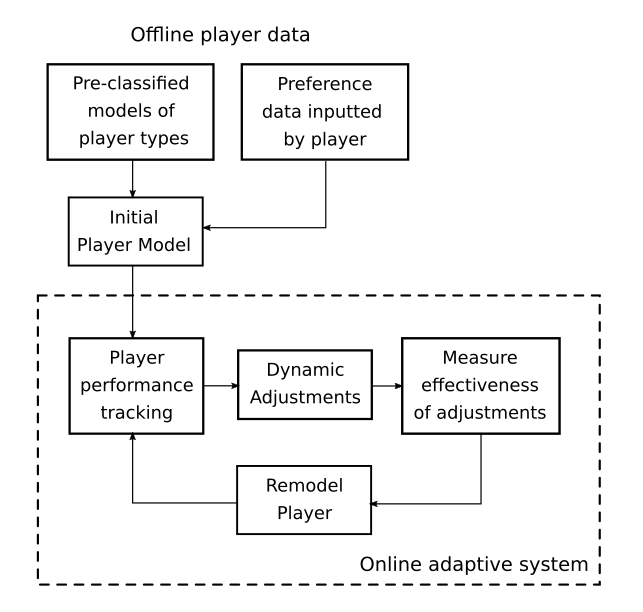
\includegraphics[width=26em]{figures/fig-dynamic-player-model.png}
    \end{center}
    \legend{Source: Diagram assembled by the authors based on visual representations in \cite{ARTICLE_DynamicPlayerModelling}.}
    \label{fig:dynamic-player-model}
\end{figure}

\section{Research on Player Experience and Difficulty in Video Games}

The objective of this work is to create a reliable system that is able to improve player experience for anyone, regardless of \emph{player profile} or \emph{player preferences}. To understand how to improve player experience, we first define what constitutes it.

In this chapter, we identify the components that constitute player experience based on previous research. We attempt to extract concrete, functional features from the subjective term \emph{experience}, and translate these features into tools to design a proper challenge for the player, as well as to avoid mistakes and misconceptions on level design.

To perform such a task, we analyze the impact of difficulty in games and its boundaries by reviewing literature on the psychology of player enjoyment. We review why the correct level of challenge can contribute to increasing levels of immersion and the overall positive experience of a player.

\subsection{Definition of Player Experience}

In the scope of this work, we evaluate \emph{Player Experience} in the specific case of Video Games. We review and relate the concepts of \emph{Usability} and \emph{User Experience} to understand how they describe the interaction between users and a systems. We study how \emph{Player Experience} differentiates from \emph{User Experience} describing the specific properties of video games in relation to conventional software.

Computer software is commonly developed with the objective of allowing an user to execute a set of tasks, determined by a clear objective and in a specific context \cite{ARTICLE_FromUsabilityToPlayability}. One of the early endeavours in the field of HCI (Human-Computer Interaction) was the efficiency of performing the \emph{task} to ensure a product's instrumental value \cite{ARTICLE_UserExperienceAResearchAgenda}.  In this line of thought, users of an application should ideally perform tasks without thinking about the application. 

Research on the interaction between people and systems in the field of HCI led to the concept of \emph{usability}, defined by \cite{ISO_ISO92411} as:

\begin{quotation}
"The extent to which a system, product or service can be used by specified users to achieve specified goals with effectiveness, efficiency and satisfaction in a specified context of use."
\end{quotation}

This definition specifies the three qualities of a usable product: \emph{effectiveness}, \emph{efficiency} and \emph{satisfaction}. We argue that while effectiveness and efficiency can be related to productivity,  satisfaction may not be fulfilled solely by productivity. For instance, an user might feel dissatisfied with the audiovisual components of an application such as its interface, even though the application perfectly satisfies the purpose of assisting in the completion of tasks efficiently.

The work of \citep{ARTICLE_UserExperienceAResearchAgenda} states that early writings on usability expressed that productivity is not primary, but only a contributor to \emph{User Experience}. The term "user experience" does not have a standard definition, but can be seen as how people interact with products and the resulting experience and emotions \cite{ARTICLE_UnderstandingExperience}. The experience is therefore a consequence of: the user's state, such as their emotions and needs; the characteristics of the product, such as usability and audiovisual aspects and the context of use, such as the environment and date.

According to \cite{ARTICLE_FromUsabilityToPlayability}, the concept of \emph{usability} is not sufficient to fully describe UX (User Experience) in relation to Video Games. The authors argue that video games are a specific type of interactive system used for leisure purposes. Thus, when evaluating quality not only instrumental values should be considered, but also non-instrumental values such as storytelling, visuals and character design. The author also introduces the concept of \emph{Player Experience}, a specialization of UX that emphasizes the specific properties of experience in games.

The author explains that Player Experience is characterized by \emph{Playability}, a concept based on Usability but with different meanings in the video game context. The proposed definition of \emph{Playability} by \cite{ARTICLE_FromUsabilityToPlayability} resembles the original Usability definition, but emphasizes the user-centric perspective and the satisfaction property:

\begin{quotation}
"Playability represents the degree to which specified users can achieve specified goals with effectiveness, efficiency and specially satisfaction and fun in a playable context of use."
\end{quotation}

This definition is further explained when the author introduces a set of seven attributes that compose Playability: \emph{Satisfaction}, \emph{Learnability}, \emph{Effectiveness}, \emph{Immersion}, \emph{Motivation}, \emph{Emotion} and \emph{Socialization}. The concepts of effectiveness and satisfaction remain present in this definition, but are specialized or complemented. Efficiency is specified as \emph{learnability} and \emph{immersion}, and the satisfaction aspect is complemented by\emph{emotion}, \emph{motivation} and \emph{socialization} to define a set of user-centred attributes. Since this work focuses on a single-player environment, we will discuss the first six attributes and evaluate which of them can be manipulated by a reliable system through AGT.

\emph{Satisfaction} is the degree of enjoyment derived from playing, characterized by \emph{fun}, \emph{disappointment} and \emph{attractiveness}. Fun is classified as the ability of a game to entertain the player whether through challenge, curiosity or competition. Disappointment refers to the feeling of disappointment of the player in relation to a game. Attractiveness encompasses any functional or aesthetic features that increases the pleasure of play such as realistic visuals, exceptional character design or interesting systems.

\emph{Learnability} is defined as the player's capacity to understand the game systems and improve their level of proficiency in relation to the game. It is categorized by \emph{Game Knowledge}, \emph{Difficulty}, \emph{Frustration}, \emph{Speed} and \emph{Discovery}. In this context, Game Knowledge refers to the player's prior expertise to the game's mechanics and environment, and influences how the player is affected by the \emph{learning curve} [FN]. Skill can be identified in the player's cognitive aspects such as strategic and analytic decision-making, or interactive aspects with efficient usage of game mechanics.

\emph{Difficulty} relates to the challenge perceived by a player in relation to their skill. The degree of difficulty can either encourage a player to improve by learning how to play or cause frustration. Frustration relates to the feeling of uneasiness when failing to complete a particular objective and is often part of the learning process. Speed refers to the pace in which new concepts are presented to players and affects the game's learning curve. Discovery refers to the techniques employed by the game to help players assimilate game content such as interfaces or level design, and directly affects the learning curve.

\emph{Effectiveness} refers to the resources necessary to entertain players, determined by \emph{Completion} and \emph{Structuring}. Completion is related to the overall percentage of players that feel motivated to reach the game's final goal. Structuring emphasizes the locality of content as when, where and how gameplay elements appear in the game. For instance, the placement of enemies and level geometry will contribute to how the player perceives and performs an objective, indirectly affecting the learning process.

\emph{Immersion} depicts the capacity of a game to be believable in a way that the player becomes involved, losing their awareness of surroundings and sense of time. The \emph{immersion} factor can be determined by \emph{Conscious Awareness}, \emph{Absorption}, \emph{Realism} and \emph{Dexterity}. Conscious Awareness is the degree to which a player is aware of the in-game outcomes of their actions, so that they can effectively plan and execute according to a situation. Absorption refers to the level of focus of a player has to a game in a given moment, and is inversely proportional to the level of focus to their real world surroundings. Realism depicts how the game's presentation influences the ease of player absorption, relying in game characteristics such as controls and game atmosphere. Dexterity relates to the ease of a player handling the game's controls and systems, so that performing in-game actions is natural and effortless.

\emph{Motivation} is the group of attributes that compel the player to perform one or various in-game actions, defined by \emph{Encouragement}, \emph{Curiosity} and \emph{Self-Improvement}. Encouragement is the level of confidence felt by a player when facing unexplored challenges. Curiosity is the degree to which a player is interested in interacting with new elements. Self-Improvement is the process of ability development and happens any time a player must overcome a challenge that is more difficult than their skill level. 

\emph{Emotion} refers to involuntary player responses to the cognitive stimulus of a video game, defined by \emph{Reaction}, \emph{Conduct} and \emph{Sensory Appeal}. Reaction consists of the emotional response of a player in relation to a series of in-game events. Conduct is the ability of a game to conduct a player through a proposed range of emotions caused by different stimuli. Sensory Appeal denotes how interesting a game is in the aesthetic perspective using different sensory channels. For instance, a game with realistic graphics and sound effects might appeal to the audiovisual sensory channel of players.

The definition of \emph{Playability} proposed by \citet{ARTICLE_FromUsabilityToPlayability} defined several attributes that categorize the characteristics of a player, the resources employed by a game and how different game aspects are able to affect a player. We argue that one of the concepts that is most frequently discussed in this work is that of  \emph{Challenge}. If challenge is presented poorly, the player might feel frustrated and discouraged to self-improve. Thus, the level of challenge must not deviate exceedingly from the level of skill by a player. In another perspective, challenge by itself can be a motivating factor for self-improvement and contribute to the overall satisfaction.  

Challenge is defined by the difficulty of an objective, the overall learning curve and player skill level. Therefore, it is directly related to how well a player learns and adapts to the game's systems. Therefore, it is imperative to comprehend how challenge fully affects players, and how learning tools such as \emph{Failure} and \emph{Punishment} are employed in game systems.

\subsection{Challenge and Flow in Games}
\label{section-challenge-flow}

Failure can be described when a player is unsuccessful in the completion of an in-game task. In the event of failure, video games punish the player with some type of progression loss or setback. In the classic Arcade-style game \emph{Tetris}, the player must replay the game from the beginning upon losing. While this approach might be acceptable in session-oriented games with no narrative progress, modern Game Design encourages the usage of less punishing setbacks such as restarting at \emph{checkpoints}. 

The perceptible change in failure outcomes suggests that punishment could be detrimental on the enjoyment of a game, depending on its gravity. The controversy of player failure and punishment requires the clarification of its purpose in games. If the only possible outcome of losing was a negative experience, the very existence of this system would be questionable.

According to \cite{ARTICLE_FearOfFailure}, failure serves the function of making players readjust their perception of a game. When a player fails performing a task, they realize the strategy that was performed is not the correct or optimal solution to a problem. The player then reevaluates the situation, analyzes what caused the failure and attempts a new strategy. This cycle provides the player an opportunity to deepen their knowledge, and encourages the creativity of new solutions.

We argue that punishment in games serves the purpose of establishing the contrast between consequences of player actions. In a simple perspective, punishment explains the rules of a game, and how a player is supposed to play it. In the game \emph{Super Mario Bros} (1985), the player has a predetermined number of lives upon starting the game, which is decreased with each death. Upon dying, the player is punished by replaying the current level. If all lives are lost, the player replays the entire game from the beginning.

The aversion to losing the progress made in a game serves as encouragement for the player to learn how to avoid defeat. In \emph{Super Mario Bros}, the player quickly learns that enemies should be avoided or beaten, and lava or bottomless pits should be evaded. If punishment mechanics did not exist, the player would simply progress by running to the right until reaching the end of a level without taking part in the proposed gameplay mechanics.

In the case of Dark Souls, punishment is used as a tool to create tension and increase player awareness. With each death, the player loses all their experience points\footnote{Experience Points are resources acquired by the player upon defeating enemies with the purpose of serving as a currency for purchasing upgrades for the player character. Such upgrades can improve the efficiency of the player in combat, or enable the player to use better equipment. In the Dark Souls game series, the Experience Points, also known as "Souls", can also be used for trading with \emph{NPCs} (Non-Player Characters) for purchasing various items which assist the player when progressing.}. If a player wishes to recover them, they must retrieve them from the same position where they were defeated. Dying again means the experience points are lost permanently. In other words, the player is forced to beat the challenges they previously failed to avoid progression loss. Death in Dark Souls can be an extremely frustrating experience, and arguably be considered as overly punishing.

Since the experience points are used to evolve the character and directly affect the outcome of future encounters, the player is encouraged to survive by any means after accumulating a reasonable amount. Upon reaching a checkpoint, the player can then spend their experience points to attain permanent attribute bonuses. Therefore, the fear of losing character progress before reaching a checkpoint reinforces the necessity of careful and strategical decision making.

While the philosophy of punishment as a tool is powerful as means of encouraging learning and adaptation, it can also be the source of anxiety and demotivation. If the punishment mechanics do not provide possibility of player evolution, they aggravate the exhaustion of repeatedly trying without success. We argue that if a game is excessively challenging to the skill level of a player, overly punishing will be the catalyst to surrender. Thus, the game system should also take in account the levels of punishment required to encourage player evolution without hindering the learning process.

In the context of video games, Challenge is an abstract concept commonly referred as the player's perception of difficulty \cite{ARTICLE_RoleOfChallenge}. If a game is considered challenging by the general public, the majority of players would agree that the game requires a high skill level to complete. Nonetheless, a game that is considered easy by the public can still be challenging to a smaller audience with less technique or experience.

The difference between the level of challenge and skill directly affects the quality of player experience. If a game is too easy to the skill level of a player, they will not feel any sense of accomplishment upon completion and will experience boredom. If a game is too hard, the player might feel overwhelmed and experience anxiety. This is supported by the Theory of Flow, proposed by \cite{BOOK_Flow}.

The Theory of Flow indicates the existence of a state of complete focus in an activity, with a high level of energy, enjoyment and fulfillment. In this state, people lose track of time and external problems. Flow is considered to be state where optimal experience takes place. The level of focus achieved in being such a state maximizes the pleasure and performance of an activity.

According to the Theory of Flow, the main components of Flow are a challenging activity, the merging of action and awareness, clear goals, immediate feedback, concentration, a sense of control, loss of self-consciousness and an altered sense of time. However, not all of them are needed for an activity to provide the user the feeling of Flow. These descriptions of Flow can be observed in games when a player becomes immersed, temporarily engaging the perspective of a virtual reality.

The Theory of Flow also states that to maintain the state of Flow, the challenge of an activity must be balanced to the abilities of the person performing it. This concept is known as \emph{Flow Channel} or \emph{Flow Zone}. This can be translated directly to the concepts of Difficulty and player Skill Level in gaming. Different players will present different Flow Channels. Hardcore players will prefer more aggressive challenge scaling in comparison to their skill, whereas Casual or Novice players will prefer a more subtle introduction to the game's complexity \cite{ARTICLE_FlowInGames}. Figure \ref{fig:flow-channel} exemplifies the \emph{Flow Channel}, where a balance of difficulty and player skill denotes the optimal conditions for player immersion and focus.

\begin{figure}
    \caption{A visual representation of the concept of \emph{Flow Channel} or \emph{Flow Zone} discussed in \cite{BOOK_Flow}.}
    \begin{center}
        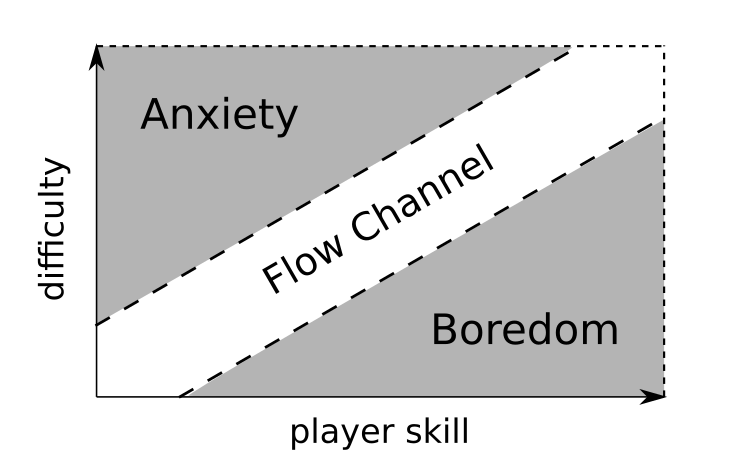
\includegraphics[width=26em]{figures/fig-flow-channel.png}
    \end{center}
    \legend{Source: Diagram assembled by the authors based on the concepts defined by \cite{BOOK_Flow}.}
    \label{fig:flow-channel}
\end{figure}

The balance between challenge and skill strongly contributes to the optimal experience of a player, and is referred to as a defining factor on the quality of a game \cite{ARTICLE_FearOfFailure}. We argue that we can balance the level of challenge through AGT. By acquiring information on the profile and preferences of a player, we can either ramp up the difficulty or encourage the learning process. Therefore, we understand that the usage of AGT can directly contribute to a positive experience.

\subsection{Learning Curve}

Another interesting concept in games is the \emph{learning curve} \cite{article_learningcurve}. The learning curve depicts how easy it is to become used to the game's mechanics and systems. Game Developers often consider the learning curve as a key reference when performing level design. The first few levels of a game should enable the player to learn each mechanic in an isolated and controlled environment, whereas the last levels of a game should be designed considering that the player has knowledge about all the mechanics proposed by the game designer, and thus should present challenges that require mastery of each mechanic to surpass. Figure \ref{fig:difficulty-curves} depicts multiple possibilities for difficulty curves as a function of player progress in a game.

\begin{figure}
    \caption{Examples of the distribution of difficulty in games as a function of player progress.}
    \begin{center}
        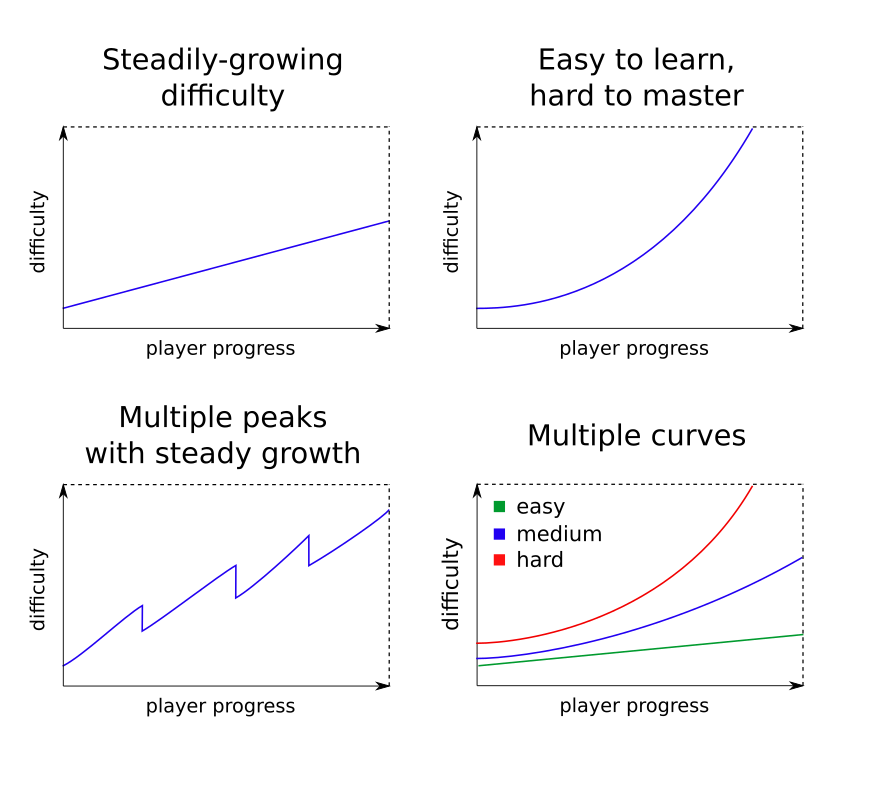
\includegraphics[width=26em]{figures/fig-difficulty-curves.png}
    \end{center}
    \legend{Source: Diagram assembled by the authors.}
    \label{fig:difficulty-curves}
\end{figure}

Perhaps the most notable example in teaching game mechanics through a concise learning curve is seen the famous game \emph{Super Mario Bros} \footnote{Super Mario Bros (Nintendo, 1985). Video Game. Nintendo Entertainment System.} in World 1-1, as addressed in \cite{video_extracreditsmario11}. In the first thirty seconds of gameplay, the player is able to learn that they must progress going to the right, that enemies must be avoided or eliminated by jumping in their heads and that special blocks hide valuable rewards such as additional lives. All the mechanics are taught without a single line of text or on-screen dialog box. Instead, the game teaches them by simply using the player's curiosity with an ingenious placement of game entities.

Some genres of games with consolidated and well-known mechanics share multiple similarities. The mechanics in such genres are proven to be one of the core constituents in their type of gameplay, and are expected by any non-novice player. One example would be the FPS (First Person Shooter) mechanics of \emph{Call of Duty: Modern Warfare}\footnote{Call of Duty: Modern Warfare (Infinity Ward, 2007). Computer Game. Microsoft Windows.}. The running, sprinting, strafing, vaulting, proning and iron-sighting mechanics were so exceptionally well done that they still remain in the most recent title of the series, \emph{Call of Duty: Black Ops 4}\footnote{Call of Duty: Black Ops 4 (Treyarch, 2018). Computer Game. Microsoft Windows.}. Other entries in the FPS genre such as \emph{Battlefield}\footnote{Battlefield 5 (DICE, 2018). Computer Game. Microsoft Windows.} also employ the same set of mechanics, which has since then become almost a requirement for the non-tactical Arcade Shooter style.

Arguably, games with the mechanics of a consolidated genre have a faster initial learning curve to any player that has played a similar game before. These games take advantage of that, and throw the player straight into the action. Within the first few minutes of playing a \emph{Call of Duty} game, the player will have faced and beaten an impressive amount of enemies. They will also confirm their proficiency by choosing exactly the difficulty level that appeals to their skill. Therefore, the veteran player of such a genre knows what to expect of the game and its standard difficulty level. They tailor their game experience to the optimal experience in the act of leisure.

We argue that Adaptive Game Technologies can also have an impact on the learning curve issue. Understanding the profile of a player before gameplay takes place can be a key factor on the decision to ramp up the initial challenge of a game, and remove or alter initial sections which only serve the purpose of teaching basic mechanics.

Thus, the learning curve should not be static, but customized to the needs of each player. If the player has already mastered the base concepts of a game, they should be encouraged to using their knowledge to the fullest. Tailoring the learning experience to each player could balance the challenges faced by the player to a more appropriate, which could possibly increase the sense of enjoyment and immersion as seen in \autoref{section-challenge-flow}.

\section{Conclusions}

Ideally, a DDA system should embrace all skill levels, be transparent and only create positive outcomes for player experience. However, the examples discussed in this section have shown us that players will often become aware of such systems and exploit them as a strategic and controllable advantage. 

%============================================================
%============================================================
%============================================================
%============================================================
%============================================================
%============================================================

%\chapter {Definition of Games, Experience and Difficulty}

%\section{A Systematic Definition of Games}

%It is possible to define digital games purely as being interactive systems, similar to some types of computer software \cite{ARTICLE_FromUsabilityToPlayability}. Whereas computer software is commonly developed with the objective of the user executing a set of tasks assisted by an automated system, video games are used for leisure purposes. Thus, it is necessary to understand what aspects constitute a game and how it differentiates from other interactive systems before defining player experience.

%Perhaps the most precise definition of games in recent academic literature is discussed in \cite{ARTICLE_TheGameThePlayerTheWorld}. Their work claims the existence of a standard for creating games that has been constant for thousands of years. While many other definitions exist, we chose the definition by \citeauthor{ARTICLE_TheGameThePlayerTheWorld} because it compares and formulates over the definitions of various authors from the history of game research. Their work also proposes specific components to their definition, and discusses the relation of game systems to their players. Thus, \citet{ARTICLE_TheGameThePlayerTheWorld} proposes the following definition of \emph{games}:

%\begin{quotation}
%"A game is a rule-based formal system with a variable and quantifiable outcome, where different outcomes are assigned different values, the player exerts effort in order to influence the outcome, the player feels attached to the outcome, and the consequences of the activity are optional and negotiable.."
%\end{quotation}

%This definition is not restricted to any types of medium. Rather, it can be applied to \emph{analog games}, digital games, sports and even gambling. The author explains that this definition is characterized by six components: \emph{Rules}, \emph{Variable and Quantifiable outcome}, \emph{Valorization of outcome}, \emph{Player Effort}, \emph{Attachment of the player to the outcome} and \emph{Negotiable consequences}.

%Games have \emph{Rules} that must be sufficiently well defined so that they are clearly understood and agreed upon by all participants. In the case of a non-electronic game, disagreement on the rules would result in the game being stopped and discussed over. In the case of digital games where the player interacts directly to the system, the developer should make the rules unambiguous and clear enough for a player to understand by their self.

%The rules of a game must provide \emph{Variable outcomes}. For example, making different choices should result in different outcomes for a player. The author also argues that if player actions do not influence the outcome of a game, then the game can not be classified as a game \emph{activity}. The game must have \emph{Quantifiable outcomes} beyond the uncertainty of discussion. If a player performs an action, it should have a clear and predefined outcome such as winning or losing points.

%Some of the possible outcomes of a game are better than others, thus creating the \emph{Valorization of the outcome}. For instance, in a multiplayer game the difference in the positivity of outcomes creates the conflict between players. Players will value most the actions which produce the better outcomes for their self interest. The author also states that there is a tendency that positive outcomes are harder to reach than negative outcomes, this being the cause of difficulty or challenge. 

%The concept of \emph{Player effort} emphasizes that player actions must influence the outcomes of a game. The author argues that the effort put in performing these actions tends to lead to an attachment of the player to the outcome, since the player would be in part responsible for the results. The \emph{Attachment of the player to the outcome} is defined as a psychologycal feature of the game activity by which the player is affected by the outcome. A player may feel happy if they win, or unhappy on loss. However, the attachment to outcome is not just related to the effort since the player can still feel happy for winning games by pure chance. The author further argues that the attachment to outcome depends on a player's attitude towards a game and is part of the game contract.

%The author defines \emph{Negotiable consequences} by discussing that games can optionally be assigned real-life consequences. The assignment can be negotiated on a per-play, per-location or per-person basis. One example for this would be gambling games where the player must bet a minimal amount before playing. The author emphasizes that some games may also have non-negotiable consequences, such as sports where a player might have an injury.

%Defining games as systems is useful in explaining the necessity of choice and consequence. It also discusses one possible argument for the motivational pull of games: the \emph{Attachment to outcome}.  While the outcomes of game systems can be motivating factors to the act of play, we argue that they are not sufficient in fully explaining player experience. For instance, \emph{horror games}[FN] might cause the feeling of uneasiness and discomfort. These types of games can also be analyzed in terms of rule-based formal systems, but one could argue that this is not the nature of their motivational pull. The definition of such games implies that the player will inevitably experience negative feelings and outcomes. To understand how negative feelings and outcomes in games can contribute to an overall positive experience, we must study what constitutes \emph{Player Experience}.

%\section{The Many Types of Difficulty}

%Traditionally, Game Design employs difficulty as a static experience \cite{article_casefordynamicdifficulty}, optionally with a fixed set of modifiers. In the Arcade Era of games, titles such as \emph{Pac-Man} \footnote{Pac-Man (NAMCO, 1980). Video Game. Arcade.} and \emph{Donkey Kong} \footnote{Donkey Kong (Nintendo, 1981). Video Game. Arcade.} started with a fixed difficulty, which increased each time the player completed a level. In the more recent Console Era of games, titles such as \emph{God of War 3} \footnote{God of War 3 (Sony, 2010). Playstation 3.} and \emph{NieR:Automata} \footnote{NieR:Automata (Platinum Games, 2017). Microsoft Windows, Playstation 4, Xbox One.} offer multiple difficulty presets. Before starting the game, the player chooses between Easy, Normal and Hard modes. The initial difficulty of any mode slightly increases with story progression by presenting new enemies, obstacles and boss fights.

%Recent games such as \emph{Dragon Quest XI} \footnote{Dragon Quest XI (Square Enix, 2017). Microsoft Windows, Playstation 4, Xbox One.} provide further customization of difficulty with selective features. Rather than choosing between predefined difficulty presets, the player will toggle one or multiple settings such as reduced experience gained from fights, tougher enemies, not being able to flee from battle and disabling the usage of protective armour. The game does not reward the player for completing the game with these settings. However, the player still achieves a better sense of accomplishment.

%The advance of selective difficulty is a step forward on appealing to the specific preferences of players. It also enables a replayability factor for experienced players, where they can attempt a harder challenge after accumulating enough experience on the mechanics of the game. 

%Another solution to difficulty is the Adaptive approach, which proposes the runtime adaptation of in-game systems to the skill level of any player. In contrast to selective difficulty systems, adaptive systems are able to work in a real-time, transparent and non-intrusive way \cite{PHD_DynamicDifficultyAdjustment}. They do not require direct player interaction with the difficulty systems, and instead rely on statistical gameplay data. In this system, a novice player is not required to select a difficulty level. The system detects which aspects of gameplay the player struggles with and adapts accordingly.

%============================================================
%============================================================
%============================================================
%============================================================
%============================================================
%============================================================

%============================================================
%============================================================
%============================================================
%============================================================
%============================================================
%============================================================

\chapter{Methodology and Results}

\section{Overview}

% About the analysis of Dark Souls

% About our implementation of Dark Souls "Core"

% About our implementation of DDA

% About the process of our Experiment

% About the results comparing to previous DDA Systems

\section{Analysis of Dark Souls}

In this section, we analyze the Game Design of our object of study to define the essential aspects behind creating a challenging action game. We argue that understanding the Game Design of \emph{Dark Souls} is crucial to the interpretation of difficulty in games. While \emph{Dark Souls} presents a wide variety of mechanics and interactions, only the basic rules required for the implementation of the combat system will be described.

\subsection{Motivation of Choice}

Dark Souls has successfully pushed the extents of challenge in Action RPGs to their limit, providing combat with a simple yet carefully designed set of core mechanics. However, the greatest capability of the \emph{Dark Souls} series, the design of its difficulty, is for some an unwelcome trait. While having enemies with simple pattern-based AI, the game punishes players heavily for making the slightest mistakes. For this reason, \emph{Dark Souls} is often mentioned as a reference to difficulty in games \cite{URL_ExploringDesignOfDarkSouls}.

The player does not fail in \emph{Dark Souls} by dying, but by giving up on finishing the game. The game design creates a cycle of experimenting, dying, learning, adapting and only then progressing through the levels. Therefore death is not considered failure, but simply the price paid for knowledge. Because of this type of punishing yet rewarding design, the special edition of the first title in the \emph{Dark Souls} series yields the subtitle "Prepare to Die Edition".

While the average action game might reward the player for beating entire armies of enemies on his own, \emph{Dark Souls} can be a rewarding experience for the player even when basic encounters are surpassed, such as surviving a battle with a single enemy. When adventuring through the tight corridors of a dungeon or dark underground caves, the player faces unknown dangers and must fight their way out. Even the weakest enemies can surprise and kill an unsuspecting player. When facing the strong opponents, dealing the finishing blow in an intense fight means the player overcame a challenge.

Understanding the design of Dark Souls is, therefore, a key component to understanding the relationship of challenge and reward.

\subsection{Overview of Game Mechanics}

\emph{Dark Souls} is for the most part presented in a Third Person Camera perspective, with the player character positioned close to the center of the screen. The Third Person perspective is distinguished by the visibility of the player character's model and actions and a slight view of their surroundings.

In comparison to First Person Camera Systems, and considering only mechanical gameplay aspects, Third Person Cameras are better suited to action games with platforming sections. In these sections, the player must have full control and awareness over the character position to avoid falling to their death. Third person perspectives also succeed in close-combat games by providing a broad view when the player deals with multiple enemies simultaneously.

However, as seen in \cite{BOOK_LevelUpTheGuideToGreat}, Third Person Cameras often have a problem of visibility in regards to the player character in tight or confined spaces of the game world, such as corridors and small rooms. The camera must be confined inside the game level boundaries to prevent inappropriate viewing of elements of the environment, such as  out-of-bounds artifacts.

In a Orbital Third Person Camera System, character movement is based upon the relationship of character position to the camera orientation \cite{BOOK_RealTimeCameras}. If the player moves forward, the character moves towards the direction the camera is facing. In Dark Souls, moving sideways also causes the camera to slightly rotate towards the direction of the movement. Therefore, if the player constantly moves horizontally without adjusting the camera, the character will move in a circle.

In situations where the camera position is invalid, the camera should reposition inside the playable bounds of the environment whenever the intended default position of the camera would be out of the limits or inside an object. According to \cite{BOOK_RealTimeCameras}, there is no standard solution to this issue. In Dark Souls, the adopted solution is to simply pull the camera closer to the player character. The relative size of the player in screen is then greatly increased and might disrupt the visualization of important gameplay elements. 

Environment elements such as columns, rocks or even non-playable characters might impair the visualization of the player character and non-player characters, thus hindering the combat capabilities of the player. In response, Third Person games with close-quarters combat often present the "Lock-On" camera as an alternative to the default.

A View Locking Camera System, such as the Lock-On Camera, overrides the orientation of a Third Person Camera by locking the orientation of the view to a "lock target". Instead of centering on the player character, the Lock-On Camera focuses on another object or position such as a non-playable character, while still offsetting the position of the player character. This allows the visualization of the two essential elements in a combat encounter: the player character and their enemy.

In the View Locking Camera System, the player movement method changes to a circular strafe relative to the lock target position. Moving sideways results in an arc-shaped motion around the target. Forward and backwards movement transposes the player character closer to or away from the target.

The Lock-On Camera is ideal for single-target combat situations, as the player can avoid enemy attacks sideways while still keeping a desirable distance to counterattack. Area of Effect attacks which affect any entity in a circular area around the enemy can also be easily avoided by moving away from the enemy. In the case of Dark Souls, the player character orientation is updated to constantly face the target, thus simplifying the process of directing attacks at enemies. Since the player character is constantly facing the direction of the target, successfully registering the attack simply requires the player to position their character in range of the target.

Dark Souls is an Action RPG with heavy focus on close-quarters combat. In contrast to other games in the genre, the combat does not present itself as fast-paced or dynamic. Instead, the game focuses on realism and slow but strategic movements. According to \cite{BOOK_DarkSoulsBeyondTheGrave}, \emph{Dark Souls} respects its predecessors such as \emph{King's Field} with a feeling of weight and impact on hits, emphasizing the necessity of players to protect themselves behind a shield.

The controls in any game of the \emph{Souls} series operate in similar fashion: each of the character's arms are controlled by separate buttons, represented by the left and right shoulder pad in a Joystick. The player can wield different one-handed equipments in each arm, or a two-handed equipment in both arms. The character will perform actions for an arm based on which equipment is equipped, such as slashing with a sword or defending with a shield. If a two-handed weapon is equipped, using the right shoulder pad button will attack and the left will defend. The most common configuration is to have a shield in the left hand, and a weapon in the right.

During play-through, the player will come across a wide variety of weapons with different attacks, but the same core functionality. Each attack requires a certain amount of \emph{Stamina}, deals a certain amount of \emph{Damage} and has a \emph{Recover Time} after the action. Certain attacks also have the chance of \emph{Staggering} an enemy. These core concepts are strategic factors the player must consider before taking action. 

\begin{itemize}

\item \emph{Damage}: the amount of health a character loses upon getting struck by an attack. This amount can be reduced or fully negated by blocking or dodging incoming attacks.

\item \emph{Health}: an attribute representing the overall physical state of a character. Numerically, it determines how much Damage a character can sustain before being destroyed.

\item \emph{Stamina}: an attribute that represents the character tiredness. Numerically, it determines the ability to perform actions in combat. Attacking, dodging and even shielding oneself against enemy attacks all have a \emph{Stamina} cost. Although \emph{Stamina} is a finite resource, it replenishes passively after the player stops performing combat actions.

\item \emph{Recover Time}: the amount of frames the player is unable to do any actions and is vulnerable to attacks after their own attack has taken place. This attribute is used to create a feeling of weight in attacks, and can be used by the player to punish slow enemies after missing an attack.

\item \emph{Stagger}: the condition where a character is unable to perform any actions and is vulnerable to attacks after getting struck by a powerful attack or a quick succession of attacks. In \emph{Dark Souls}, this condition is especially cruel to the player, since after losing a significant amount of health the player is still susceptible to a follow-up attacks, without the ability to defend their self.

\end{itemize}

In general, Heavy attacks are slower and cost the most Stamina, but deal the highest damage and \emph{Stagger} the enemy. Light attacks are faster and can be linked for a quick succession of attacks, but deal individually less damage while having a low chance of causing \emph{Stagger}.

As means of defense, a player can Block, Dodge, Parry or simply move away from an attack. Blocking requires the player to have their shield lifted at the time of the attack. Each block costs an amount of Stamina based on the power of the attack and the character's resistances. If an enemy attack is too powerful and the character does not have the required Stamina, they may still enter a Stagger condition. Out of all the defensive actions, Blocking is the safest and least skill dependent, since it will only fail if the attack hits the back of a character. While blocking, the player will replenish Stamina at a reduced rate.

Dodging can be performed by rolling in the right direction with precise timing. While costing Stamina, succeeding in this action completely negates the damage of an attack, ignoring how powerful it is. Upon failing, the character will take full damage. Thus, this action should be performed with care and heavily depends on the player reflexes.

Similarly to Dodging, Parrying can be performed with precise timing to deflect an enemy attack and destabilize the enemy. The player can then perform a riposte attack, a powerful move that adds a considerable amount of damage. Failing a Parry will cause the player to take full damage of the attack. Parrying is harder than dodging, since time window to perform the action is considerably smaller. Thus, Parrying is a high-risk high-reward action, and can also be considered an offensive move.

However, Blocking, Parrying and Dodging require the usage of Stamina, a valuable resource which is also required to perform offensive moves. If a player only blocks incoming attacks, their Stamina will not replenish quickly enough to sustain attacks indefinitely. Moreover, if a player faces multiple enemies, blocking can sustain even less attacks, and quickly deplete the player Stamina. Dodging and Parrying are timing dependent, and thus prone to mistakes and heavy punishment. If players repeatedly try to perform the same defensive action, they will often find themselves cornered, without Stamina and vulnerable to fatal blows. Experienced players have the knowledge of when they should perform none of these actions, instead simple moving away and creating space for favorable counterattack opportunities.

\subsection{Artificial Intelligence}

Upon the research conducted in the creation of this work, no official information on the implementation of the AI in Dark Souls was discovered. According to \citeonline{YT_DarkSoulsSimpleAI}, some sources indicate a \emph{Hierarchical Task Planning Network System}, but an analysis of the in-game enemy actions provides no support to this claim. However, by multiple tests and playthroughs, it was possible to reverse engineer the behavior of enemies and suggest a replication formulae in the implementation of this work.

Non-player characters often share similar behavioral patterns in Dark Souls. While the actions of a humanoid NPC might differ from a quadruped, their overall behavior upon player presence is the same. The NPC stands idle until receiving interaction from their sensors, such as the player stepping into their line of sight. At that point, the enemy will either attack at range, if using a bow or spell, or rush towards the player and attack in close-quarters.

Enemies wearing a shield will commonly attempt to defend themselves when the player repeatedly attacks. The defense stance can be punished by the player when they perform a kick or by attacking from behind. In other occasions, a low health enemy might evade attacks or even heal theirself. Most of these strategies are predictable, even when there is a variability in the patterns used.

Ultimately, the AI of Dark Souls is simplistic, but sufficient for the objectives proposed by the developer. The predictability of this system can be considered a favorable factor for a player learning how to overcome an enemy. This simplicity is not perceivable by the player in the first playthrough, since the player will struggle with the challenging aspects of the level design. In addition, Dark Souls present its enemies as being overtly strong in comparison to the player. A slight mistake might cause the player to endure punishing amounts of damage, thus creating the illusion of a difficult opponent.

The perception of strength in Dark Souls's enemies carries similarities to the development of the original \emph{Halo} by Bungie. According to \citeonline{URL_IllusionOfIntelligence}, players perceived the smartness of an enemy based on their endurance and damage dealt to the player. Simply increasing the Health points of an enemy enhanced the first perception of enemies intelligence for playtesters. This perception of toughness could shadow the lack of intelligence of an enemy in a first playthrough. However, as the player repeatedly faces the same enemy upon countless deaths, this illusion is gradually faded.

\subsection{Level Design}

According to \cite{BOOK_LevelDesignConcept}, Level Design can be defined as an interpretation of Game Design. The Level Designer must understand the rules of a game and determine how a player is confronted by them. It can be argued that Game Design represents the theoretical part of a game, whereas Level Design applies it in practice.

Level Design determines the layout of a location, the placement of enemies, the gameplay objects and the environmental hazards. In a sense, Level Design can be seen as a means of expressing Game Design through an exploration narrative. Therefore, a game developer must consider what experiences the player is supposed to face in a section before tackling on its design.

In the case of Dark Souls, the world takes place in an open, interconnected and vertically stacked map layout. When projecting this layout on a two-dimensional chart, it resembles the format of a spiral. This type of map layout is radically different than other games in the genre such as \emph{The Elder Scrolls V: Skyrim} \footnote{The Elder Scrolls V: Skyrim (Bethesda Game Studios, 2011). Computer Game. Microsoft Windows.}, which presents  dungeon maps as horizontally spaced and linear paths.

By journeying through the world, the player will come across castles, dungeons, caves, and fortresses. It is more frequent to find oneself in small passageways than open areas, the latter being used more often in \emph{boss fights}. The need of constantly turning left and right, ascending stairs and descending through dark passages gives the developers numerous places to hide enemies and traps in. Thus, the player often faces threats such as being assaulted by an unseen enemy, getting hit by a trap or even falling to their death.

Each and every enemy the player faces has the potential to generate a difficult encounter. An enemy that is considered weak can still take away a considerable amount of Health from the player. However, enemies are commonly vulnerable after performing an attack, and thus open for an instant kill. Therefore, the player has the possibility of optimizing their play style by spotting enemies ahead of time, planning on how to exploit weaknesses and only then performing the action.

The strength of a \emph{Souls}-like game isn't just its combat. When every little bit of a level can be threatening, it encourages the player to experience the atmosphere and story of the world. The careful placement of enemies, traps and pitfalls in creative fashion constitutes the core of \emph{Dark Souls} Level Design.

A Dark Souls player is encouraged to memorize whole map sections to progress withstanding minimal damage. The constant feeling of danger increases the tension and maintains the player aware of their situation to survive. According to \citeonline{YT_EvolutionOfDarkSoulsLevelDesign}, the Level Design in  Dark Souls is the main contributor to the player immersion in the game's narrative.

However, the pitfalls and traps of Dark Souls can be spotted ahead of time if the player decides to maintain a slow pacing an pay attention to their surroundings. This characteristic makes the seemingly unfair encounters beatable. Groups can be separated into smaller sizes by luring enemies one by one. The environment traps can be used against the enemies, if the player lures the target to the area of effect. Enemies can be pulled from their territory into a safer and player-controlled position.

Spiral level designs can also feature alternate routes and shortcuts. Since the player is constantly facing the danger of losing Experience Points upon dying, the Spiral layout provides the player with shorter paths and less risk when returning to safe zones. In the same philosophy, the game will often contain shortcuts from safe zones to later attained areas. These shortcuts must be unlocked by reaching a certain location and performing an action, such as finding the key to a locked gate. This Level Design technique is commonly known as \emph{gating} \cite{BOOK_LevelUpTheGuideToGreat}.

\subsection{The "Pain Points" of Dark Souls for Beginner-Level Players}

\section{System Architecture and Design Decisions}

\subsection{Tools, Frameworks and Assets}

% Motivation for using Unity3D
% - A complete framework that is widely used in the industry, and is able to achieve AAA quality products with current examples in the industry;
\sepfootnotecontent{fn-triple-a}{AAA (pronounced "triple A") games are an informal classification of video games distributed by major publishers and distinguished by large development and marketing budgets. In general, the term is used to represent the games that are supposed to achieve the highest standard of quality and content in video games.}
\sepfootnotecontent{fn-genshin-impact}{Genshin Impact (miHoYo, 2020). Video Game. Android, iOS, Windows, PlayStation 4, Playstation 5, Nintendo Switch.}
\sepfootnotecontent{fn-escape-tarkov}{Escape from Tarkov (Battlestate Games, 2017). Computer Game. Microsoft Windows.}
\sepfootnotecontent{fn-hollow-knight}{Hollow Knight (Team Cherry, 2017). Video Game. PlayStation 4, Nintendo Switch, Xbox One, macOS, Linux, Microsoft Windows.}
\sepfootnotecontent{fn-ghost-tale}{Ghost of a Tale (SeithCG \& Plug In Digital, 2016). Video Game. PlayStation 4, Nintendo Switch, Microsoft Windows, Xbox One.}
\sepfootnotecontent{fn-cuphead}{Cuphead (Studio MDHR Entertainment Inc., 2017). Video Game. PlayStation 4, Nintendo Switch, Xbox One, Microsoft Windows, macOS.}

Unity is widely used in the video games industry, with a feature-rich framework that supplies game developers with tools to achieve AAA\sepfootnote{fn-triple-a} quality products. Some examples of successful games implemented under Unity include Genshin Impact\sepfootnote{fn-genshin-impact}, Escape from Tarkov\sepfootnote{fn-escape-tarkov}, Hollow Knight\sepfootnote{fn-hollow-knight}, Ghost of a Tale\sepfootnote{fn-ghost-tale} and Cuphead\sepfootnote{fn-cuphead}.
% - A concise integrated editor that can be used for map editor, project folder organization, game data management;
% - A general API that provides the tools to implement virtually any type of game;
% - Possibility to deploy in multiple platforms (Windows, Linux, macOS) with minimal changes in source code;
% - Possibility to import free and paid assets from the Unity Asset Store for 3D Models, Animations, Sounds, UI Elements, Shaders, Post-Processing Effects, Visual Effects;
% - Possibility to import plug-and-play APIs and systems such as Cinematic Camera behavior controllers, Third person Movement Controllers and Universal Input Device Managers that can be easily integrated into the project and development workflow;
% - Possibility to import and integrate multiple development tools that are tailored to the specific needs of the product being developed, such as data serialization utilities, map editor utilities, telemetry and database management tools and visual effect creation tools;
% - Authors had previous familiarity with the engine from personal and professional experience;

The final deciding factor for the choice of Unity as a development platform was the previous personal and professional background of the authors with the engine, having implemented a wide variety of 2D and 3D Games, VR Serious Games and data visualization tools under Unity. The familiarity with the provided APIs, along with the knowledge of how to achieve a steady and concise workflow permitted the authors to plan a robust architecture and select the appropriate tools to implement the core features of Dark Souls with an acceptable quality in comparison to the original game.

% Cinemachine

% Assets
% 3D Models, animations and sound assets were selected based on trying to replicate the same general 'feel' of Dark Souls


% Table showing Asset Name, Type, Size, Price, Path in Project
Table \ref{tab:table1} shows a list of Assets gathered from the Unity Asset Store for the assembly of this project, along with the appropriate extraction paths for the assets to work with the source code.

\begin{table}[h!]
  \begin{center}
    \caption{Assets used in the implementation of 'Bright Souls'.}
    \label{tab:table1}
    \begin{tabular}{ m{10em} m{20em} } % alignments
    
      \textbf{Name}                 & \textbf{Path in Project}                                 \\

      \hline \multicolumn{2}{l|}{\textbf{3D Models}}                                           \\ \hline
      Fantasy Dungeon               & \texttt{../Assets/Asset Store/3D/FantasyDungeon/}        \\ \hline
      Skeleton Zombies              & \texttt{../Assets/Asset Store/3D/StudioNewPunch/}        \\ \hline
      The Blacksmith: Characters    & \texttt{../Assets/Asset Store/3D/Challenger Character/}  \\

      \hline \multicolumn{2}{l|}{\textbf{Animations}}                                          \\ \hline
      ZOMBIE Starter Animation Pack & \texttt{../Assets/Asset Store/3D/Zombie\_01\_v25/}       \\ \hline
      Sword and Shield Animset Pro  & \texttt{../Assets/Asset Store/3D/SwordShieldAnimsetPro/} \\ \hline
      Longsword Animset Pro         & \texttt{../Assets/Asset Store/3D/LongswordAnimsetPro/}   \\

      \hline \multicolumn{2}{l|}{\textbf{Sound Effects}} \\ \hline
      Axe Swing \& Damage Sounds    & \texttt{../Assets/Asset Store/Audio/Axe Swing \& Damage Sounds/}             \\ \hline
      Dark Fantasy Audio            & \texttt{../Assets/Asset Store/Audio/Dark Fantasy Studio- Shadows Guild mp3/} \\ \hline
      Medieval Fantasy 2 Audio      & \texttt{../Assets/Asset Store/Audio/Medieval Fantasy Audio Bundle 2/}        \\ \hline
      Universal Sound FX            & \texttt{../Assets/Asset Store/Audio/Universal Sound FX/}                     \\ 

      \hline \multicolumn{2}{l|}{\textbf{Visual Effects}}                                   \\ \hline
      Pseudo-Volume Blood Effects   & \texttt{../Assets/Asset Store/VFX/KriptoFX/BloodFX/}  \\ \hline
      Smoke \& Ember FX             & \texttt{../Assets/Asset Store/VFX/Smoke \& Ember FX/} \\ \hline
      Unity Particle Pack           & \texttt{../Assets/Asset Store/VFX/UnityParticlePack/} \\

      \hline \multicolumn{2}{l|}{\textbf{UI Elements}} \\ \hline
      PC \& Consoles Buttons Icons  & \texttt{../Assets/Asset Store/UI/PC \& Consoles Controller Buttons Icons Pack/} \\ \hline
      RPG \& MMO UI 5               & \texttt{../Assets/Asset Store/UI/RPG and MMO UI 5/} \\

      \hline \multicolumn{2}{l|}{\textbf{Editor Plugins}} \\ \hline
      Odin Inspector                & \texttt{../Assets/Plugins/Sirenix/} \\

    \end{tabular}
  \end{center}
\end{table}

\subsection{Gameplay Mechanics and Systems}

\subsection{Artificial Intelligence}

Test.

% Figure: Melee enemy AI State Machine
\begin{figure}[!h]
    \caption{An example of the State Machine that represents a Melee Enemy AI Agent. Each state holds its own behavior.}
    \begin{center}
        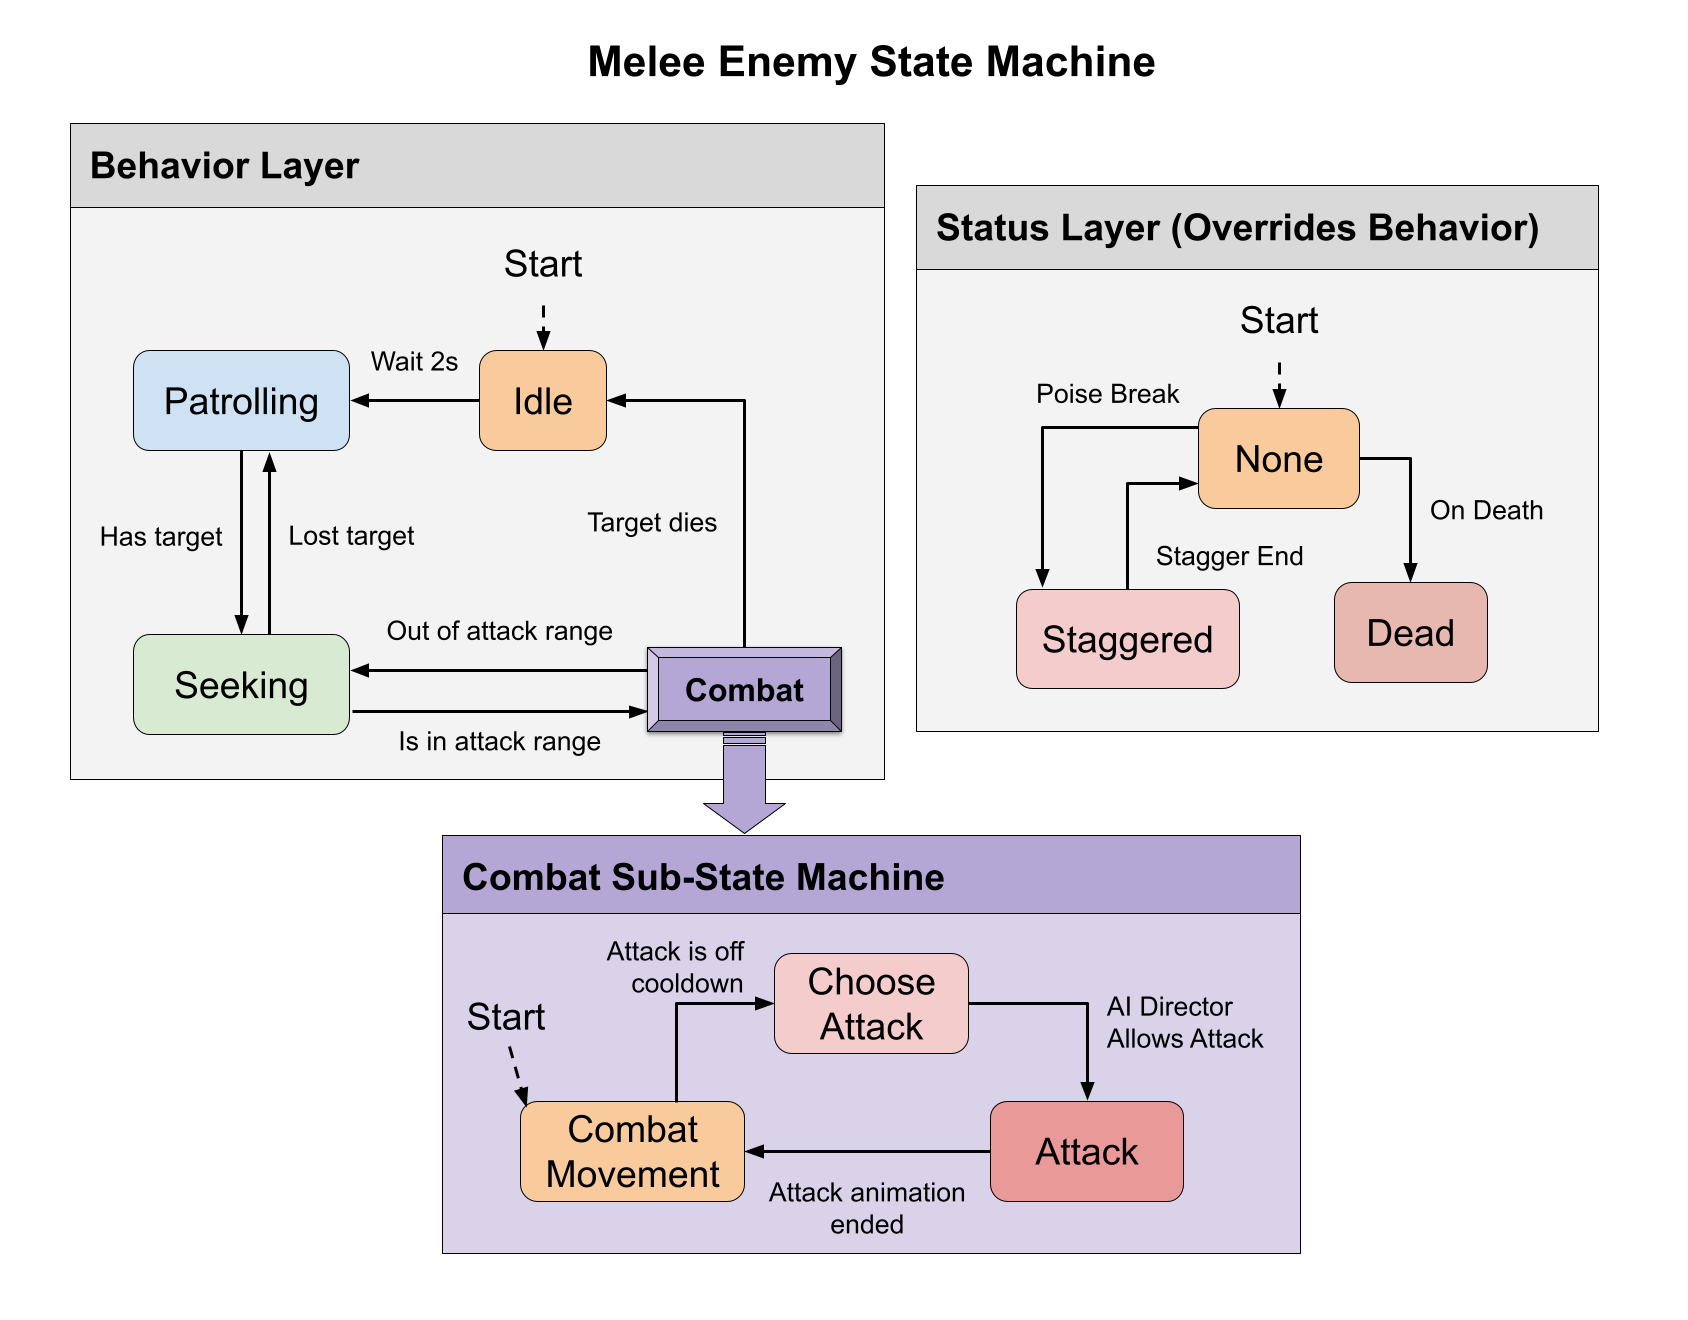
\includegraphics[width=40em]{figures/fig-melee-ai-state-machine.png}
    \end{center}
    %\legend{Source: Diagram by authors.}
    \label{fig:ex1}
\end{figure}

\subsection{Telemetry and Performance Tracking}

\subsection{Dynamic Adjustments}

\section{Experimentation Model}

\subsection{Methodology}

\subsection{Results and Analysis}

\section{Conclusions}

% limitations

% comparison with previous work

%============================================================
%============================================================
%============================================================
%============================================================
%============================================================
%============================================================

\chapter{Discussion}

\section{Overview}

\section{Contributions}

\section{Limitations and Problems}

%============================================================
%============================================================
%============================================================
%============================================================
%============================================================
%============================================================

\chapter{Conclusion}

\section{Limitations}

\section{Future Work}

%============================================================
%============================================================
%============================================================
%============================================================
%============================================================
%============================================================

% References

\bibliographystyle{abntex2-alf}
\bibliography{biblio}

\end{document}
